\documentclass{article}

\usepackage{styles/aprox}
\usepackage[latin1]{inputenc}
\usepackage[brazil]{babel}
\usepackage{indentfirst}
\usepackage{graphicx}

%--------------------------------------------------------
%\usepackage{amsmath}%
%\usepackage{amsfonts}%
%\usepackage{amssymb}%

\newtheorem{theorem}{Teorema}
\newtheorem{acknowledgement}{Aviso}
\newtheorem{algorithm}{Algoritmo}
\newtheorem{axiom}{Axioma}
\newtheorem{case}{Caso}
\newtheorem{claim}{Claim}
\newtheorem{conclusion}{Conclus�o}
\newtheorem{condition}{condi��o}
\newtheorem{conjecture}{Conjectura}
\newtheorem{corollary}{Corol�rio}
\newtheorem{criterion}{Crit�rio}
\newtheorem{definition}{Defini��o}
\newtheorem{example}{Exemplo}
\newtheorem{exercise}{Exerc�cio}
\newtheorem{lemma}{Lema}
\newtheorem{notation}{Nota��o}
\newtheorem{problem}{Problema}
\newtheorem{proposition}{Proposi��o}
\newtheorem{remark}{Observa��o}
\newtheorem{solution}{Solu��o}
\newtheorem{summary}{Sum�rio}
%--------------------------------------------------------

\hyphenation{apro-xi-ma-cao}
\hyphenation{ca-mi-nho}
\hyphenation{re-la-xa-cao}
\hyphenation{pro-ble-ma}
\hyphenation{se-me-lhan-te}

\newcommand{\rcsp}{\textsc{RCSP}}
\newcommand{\fptas}{\textsc{FPTAS}}

\title{
	\vspace{2.5cm}
	{\small EXAME DE QUALIFICA��O}\\
	{\small MESTRADO EM CI�NCIA DA COMPUTA��O\\}
	\vspace{0.3cm}
	{\bf Caminhos M�nimos com Recursos Limitados}
}
\author{
	Joel Silva Uchoa\\
	Orientador: Carlos Eduardo Ferreira
	\vspace{0.5cm}
	\\{\small DEPARTAMENTO DE CI�NCIA DA COMPUTA��O}\\
	{\small INSTITUTO DE MATEM�TICA E ESTAT�STICA}\\
	{\small UNIVERSIDADE DE S�O PAULO}
}

\begin{document}
\maketitle
\newpage

\section{Introdu��o}

Um problema bastante conhecido � o de escolher uma rota para se fazer 
uma viagem, tal que a rota minimize a dist�ncia 
do percurso. Nesta forma b�sica, esse problema � o problema de caminho 
m�nimo em grafos onde as arestas s�o poss�veis trechos, valorados por 
seu comprimento. Algumas vezes um caminho m�nimo desta forma � bom, 
outras vezes n�o. Existem ocasi�es, onde tal caminho possui propriedades
indesej�veis. Por exemplo, alguns trechos podem ter tr�fego denso e nos 
fazer perder muito tempo na travessia, ou existem muitos ped�gios com taxas
que, acumuladas pelo caminho, v�o exceder o dinheiro que temos dispon�vel.
Isso nos leva a considerar um ou mais par�metros adicionais para a escolha
do caminho. Os casos mais comuns de par�metros a considerar 
envolvem o consumo de recursos
em um or�amento que limita a quantidade dispon�vel desses
recursos. Um caminho m�nimo com essas limita��es adicionais � chamado de
{\bf caminho m�nimo com recursos limitados } 
({\it resource constrained shortest path - RCSP}) \cite{BC89}. 

\begin{problema}{\rcsp($G, s, t, k, r, l, c$)} 
Como par�metros do problema s�o dados:
\begin{itemize}
\item\ um grafo dirigido $G=(V,A)$,
\item\ um v�rtice origem $s \in V$ e um v�rtice destino $t \in V$, $s \neq t$,
\item\ um n�mero $k \in \mathbb{N}$ de recursos dispon�veis $\{1,\dots,k\}$,
\item\ o consumo de recursos $r^i_a \in \mathbb{N}_0$ de cada arco 
de $G$ sobre os  $k$ recursos dispon�veis, $i = 1, \dots, k$, $a \in A$,
\item\ o limite $l^i \in \mathbb{N}_0$ que dispomos de cada recurso, 
$i = 1, \dots, k$,
\item\ o custo $c_a \in \mathbb{N}_0$, para cada arco, $a \in A$.
\end{itemize}

O consumo de um recurso $i$, $i = 1, \dots, k$ em um $st$-caminho $P$ � 
$r^i(P) = \sum_{a \in P}{r^i_a}$. Um $st$-caminho $P$ � 
limitado pelos recursos $1, \dots, k$ se este consome n�o mais que o limite
dispon�vel de cada recurso, ou seja, se $ r^i(P) \leq l^i$, $i = 1, \dots, k$.
O custo de um $st$-caminho $P$ � $c(P) = \sum_{a \in P}{c_a}$.
O problema \rcsp\ consiste em encontrar o caminho limitado pelos recursos de
menor custo.

\end{problema}

Usaremos no decorrer deste trabalho $n = |V|$ e $m = |A|$. Quando
estivermos tratando de um contexto onde existe apenas um recurso, ou seja,
$k = 1$, usaremos apenas $l$ para representar $l^1$ e apenas $r_a$ para
representar $r^1_a$. 


\section{Hist�rico do Problema}

Os primeiros a apresentarem resultados sobre o problema foram 
Witzgall e Goldman 1965 \cite{WG65}. Joksch 1966 \cite{JO66}, 
trabalhando de forma independente, apresentou um resultado similar 
ao resultado de Witzgall e Goldman 1965 \cite{WG65} (veja tamb�m Lawler 1976 \cite{LA76}). 
Todos esses autores apresentaram algoritmos baseados em programa��o 
din�mica com complexidade pseudopolinomial, com recorr�ncias similares. 
A partir de ent�o,
o problema tem recebido grande aten��o de diversos pesquisadores.

Temos v�rios algoritmos exatos propostos ao longo do tempo para o \rcsp.
Dentre eles, cronologicamente, podemos citar Joskch 1966 \cite{JO66}, 
Lawler 1976 \cite{LA76}, Handler e Zang 1980 \cite{HZ80}, Aneja, Aggarwal 
e Nair 1983 \cite{AAN83}, Henig 1985 \cite{HE85}, Beasley e 
Christofides 1989 \cite{BC89}, Hassin 1992 \cite{RH92}. 
Os algoritmos descritos em \cite{HZ80} e \cite{BC89} usam uma relaxa��o 
lagrangeana da formula��o mais usual do \rcsp\ por programa��o linear. 
Vale ressaltar ainda que \cite{BC89} usa o m�todo de subgradiente
para resolver, aproximadamente, a relaxa��o lagrangeana.
Temos ainda Mehlhorn e Ziegelmann 2000 \cite{KM00}, que 
apresenta a abordagem do envolt�rio ({\it hull approach}), um
algoritmo combinat�rio para resolver uma relaxa��o de uma outra representa��o 
do \rcsp\ como um problema de programa��o linear.

Al�m dos algoritmos exatos, tamb�m surgiram algoritmos de aproxima��o.
Warburton 1987 \cite{WA87} desenvolveu um \fptas\ ({\it fully polynomial-time approximation scheme}) 
para o problema. Hassin 1992 \cite{RH92}, al�m de apresentar um algoritmo pseudo-polinomial, 
apresentou melhoras ao resultado de Warburton e tamb�m prop�s
um outro \fptas\ para o problema. Temos ainda mais um \fptas\ proposto por
Phillips 1993 \cite{PH93}.





\section{Complexidade}

O problema \rcsp\ � NP-dif�cil mesmo para o caso em que existe apenas um
�nico recurso (\cite{HZ80} \cite{GJ79}). N�s podemos reduzir um problema 
NP-dif�cil bem conhecido a ele, o {\bf problema da mochila} ({\it knapsack}), 
definido a seguir.

\begin{problema}{\textsc{Mochila}(N,w,v,d)}
Como par�metros do problema s�o dados:
\begin{itemize}
\item\ Um conjunto de itens $N = \{1, \dots, n\}$,
\item\ pesos $w_i \in \mathbb{N}$, $i = 1, \dots, n$, para esses itens,
\item\ valores $v_i \in \mathbb{N}$, $i = 1, \dots, n$, para esse itens,
\item\ um peso limite $d \in \mathbb{N}_0$.
\end{itemize}
O peso de um subconjunto $I \subseteq N$ �
$w(I) = \sum_{i \in I}{w_i}$, e seu valor � 
$v(I) = \sum_{i \in I}{v_i}$. O problema \textsc{Mochila} consiste em
encontrar um subconjunto de itens com valor m�ximo, cujo peso n�o excede
o limite $d$.
\end{problema}

\begin{teorema}{} O \rcsp\ � NP-dif�cil.
\end{teorema}

\begin{prova} A prova se d� pela redu��o do problema \mochila\ ao \rcsp.
Vamos tomar uma inst�ncia $I$ do problema \mochila. N�s podemos
construir uma inst�ncia $I'$ para o \rcsp\ como se segue:
\begin{itemize}
\item $V := N \cup \{0\}$.
\item $A := A_1 \cup A_2$.
    \begin{itemize}
        \item $A_1 := \{(i-1,i): i=1,\dots,n\}$,
        \item $A_2 := \{(i-1,i): i=1,\dots,n\}$.
    \end{itemize}
\item $s := 0$, $t := n$.
\item $k = 1$.
\item $l := d$.
\item 
$
	r_a := \left\{
	\begin{array}{ll}
		\begin{array}{ll}
			w_i, & \text{se } a \in A_1, \\
			0, & \text{caso contr�rio}
		\end{array} & \text{para todo } a \in A.
	\end{array}
	\right.
$
\item
$
	c_a := \left\{
	\begin{array}{ll}
		\begin{array}{ll}
			M - v_i, & \text{se } a \in A_1, \\
			M, & \text{caso contr�rio}
		\end{array} & \text{para todo } a \in A.
	\end{array}
	\right.
$

\end{itemize}

\begin{figure}[h!]
    \centering
        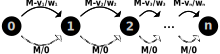
\includegraphics[scale=1.5]{figuras/grafo_rscp_mochila.png}
    \caption{\it Os arcos preenchidos s�o os arcos de $A_1$ e os 
        tracejados de $A_2$. O r�tulo de cada arco $a$ representa $c_a/r_a$.}
    \label{fig:rscp_mochila}
\end{figure}


A constante $M$ pode ser definida como um grande inteiro 
de tal forma que $M-v_i$, para qualquer $i$, seja n�o negativo.
Por quest�o de praticidade, vamos convencionar que representaremos um
arco $(i-1,i) \in A_1$ como $a^1_i$ e um arco $(i-1,i) \in A_2$
como $a^2_i$.

Como $s=0$, $t=n$; podemos ver que qualquer $st$-caminho $P$ 
em $G = (V,A)$ cont�m 
ou $a^1_i$ ou $a^2_i$, $i=1,\dots,n$. Vamos dividir
os arcos de $P$ em dois conjuntos $X$ e $Y$, onde $X$ cont�m os arcos em
$P$ que est�o em $A_1$, e $Y$ cont�m os demais arcos. A partir 
de $X$, vamos definir um subconjunto $S \subseteq N$,
tal que $i \in S$ se e somente se $a^1_i \in X$. 
Com isso,

\begin{equation}
\begin{array}{rcl}
c(P) & = & \displaystyle\sum_{a^1_i \in X}{(M-v_i)} + \displaystyle\sum_{a^2_i \in Y}{M}\\
     & = & n \cdot M - \displaystyle\sum_{a^1_i \in X}{v_i}\\
     & = & n \cdot M - v(S)
\end{array}
\end{equation}

\begin{equation}
\begin{array}{rcl}
r(P) & = & \displaystyle\sum_{a^1_i \in X}{w_i} + \displaystyle\sum_{a^2_i \in Y}{0} \\
     & = & \displaystyle\sum_{a^1_i \in X}{w_i} \\
     & = & w(S)
\end{array}
\end{equation}

Da�, conclu�mos que todo subconjunto $S \subseteq N$ cont�m um $st$-caminho $P$ associado, e 
vice-versa, por meio da equival�ncia 
$i \in S \Leftrightarrow a^1_i \in P$.
Pelas equa��es $(1)$ e $(2)$, um conjunto $S$ e um caminho $P$ associados, 
possuem $r(P)=w(S)$
e $c(P) = n \cdot M - v(S)$. E da� temos dois resultados:
\begin{displaymath}
\begin{array}{rcl}
r(P) \leq l & \Longleftrightarrow & w(S) \le d$$\\
\text{ minimizar } c(P) & \Longleftrightarrow & \text{ maximilizar }v(S)
\end{array}
\end{displaymath}
\end{prova}




\subsection{Algoritmos Exatos}


\begin{frame}
    \frametitle{Algoritmos Exatos}
    
    Por praticidade, para os algoritmos a seguir, 
    \begin{itemize}
        \item vamos assumir que $s = 1$ e $t = n$;
        \item vamos descrever para a vers�o com um �nico recurso.
    \end{itemize}
    Mas os algoritmos podem ser facilmente generalizados.  

\end{frame}


\subsubsection{Programa��o Din�mica}

\begin{frame}

\frametitle{Algoritmo A} 

    {\small
    Definimos $f_j(r)$ como sendo o custo de um caminho de $1$ a $j$ com menor 
    custo, que consome no m�ximo $r$ unidades de recurso, 
    e assim temos a recorr�ncia:
    \begin{displaymath}
        f_j(r) = \left\{
        \begin{array}{lcl}
            0, & &\text{se } j=1  \\ & & \text{ e } r=0,\dots,l\\
             & & \\
            \infty, & & \text{se } j=2,\dots,n  \\ & & \text{ e } r=0\\
             & & \\
            \min\left\{f_j(r-1), \displaystyle\min_{k|r_{kj}\leq r}\{f_k(r-r_{kj})+c_{kj}\}\right\}, & & \text{se } j=2,\dots,n  \\ & & \text{ e } r=1,\dots,l\\
        \end{array}
        \right.
    \end{displaymath}

    Podemos implementar um algoritmo que computa o valor de um caminho �timo 
    $OPT = f_n(l)$ em tempo $O(nml)$. 
    }

\end{frame}

\begin{frame}

\frametitle{Algoritmo B} 

    Definimos $g_j(c)$ como sendo o custo do caminho que consome
    menos recurso de $1$ a $j$, e tem custo m�ximo $c$. Assim, temos a recorr�ncia:
    {\scriptsize
    \begin{displaymath}
        g_j(c) = \left\{
        \begin{array}{lcl}
            0, & &\text{se } j=1 \\ & &  \text{ e } c=0,\dots,OPT\\
             & & \\
            \infty, & & \text{se } j=2,\dots,n \\ & & \text{ e } c=0\\
             & & \\
            \min\left\{g_j(c-1), \displaystyle\min_{k|c_{kj}\leq c}\{f_k(c-c_{kj})+r_{kj}\}\right\}, & & \text{se } j=2,\dots,n \\ & & \text{ e } c=1,\dots,OPT\\
        \end{array}
        \right.
    \end{displaymath}
    }

    {\small
    $OPT$ pode ser expresso como $\min\{c\ |\ g_n(c) \le l\}$. 
    Devemos computar $g$ iterativamente, at� o primeiro valor $c'$ tal que $g_n(c') \le l$. 
    S� ent�o teremos o conhecimento do valor $OPT = c'$. 
    A complexidade do algoritmo sugerido acima � $O(nmOPT)$.
    }

\end{frame}



\subsubsection{Relaxa��o Lagrangeana}

\begin{frame}
    \frametitle{Relaxa��o Lagrangeana - Primal}


    \begin{itemize}
        \item Algoritmo proposto por Handler e Zang \cite{HZ80}.
    \end{itemize}

    {\small
    Inicialmente, vamos apresentar uma formula��o para o problema \rcsp\ usando programa��o linear. 
    Nela teremos uma vari�vel $x_{ij}$ para cada $(i,j)\in A$, $x_{ij} = 1$ significa
    dizer que o arco $(i,j)$ est� na solu��o e $x_{ij} = 0$
    o contr�rio.
    }
    {\scriptsize
    \begin{linearprogramwlabel}{(P)}
        \mbox{minimize}
            & c(x) & = & \displaystyle\sum_{(i,j) \in A} c_{ij}x_{ij} \\
        \mbox{sujeito a}
            &\displaystyle\sum_{j}{x_{ij}} - \displaystyle\sum_{k}{x_{ki}} &=& \left\{ 
                \begin{array}{rl}
	             1, & \text{se } i = 1\\
                     0, & \text{se } i = 2,\dots,n-1\\
                    -1, & \text{se } i = n\\
       		\end{array} 
        	\right. & (1)\\
    	&\displaystyle\sum_{(i,j) \in A} r_{ij}x_{ij} &\le& l & (2)\\
    	& x_{ij} & \in & \{0,1\},\ (i,j) \in A & (3)

    \end{linearprogramwlabel}
    }

\end{frame}

\begin{frame}
    \frametitle{Relaxa��o Lagrangeana - Primal}

    \begin{itemize}

        \item A restri��o $(3)$ � respons�vel por delimitar os
                poss�veis valores que um componente do vetor $x$ pode assumir.
        \item A restri��o $(1)$, por sua vez, � respons�vel por garantir que
                para um vetor $x$ ser solu��o vi�vel do problema, ele deve ``conter'' um caminho
                do v�rtice $1$ ao v�rtice $n$. 
        \item A restri��o $(2)$ nos garante
                que o conjunto de arcos induzido por um vetor $x$ vi�vel, n�o excede os
                recursos dispon�veis.
    \end{itemize}

\end{frame}

\begin{frame}
    \frametitle{Relaxa��o Lagrangeana - Primal}

    Vamos definir $\cal{X}$ denotando o conjunto de vetores $x$ que satisfazem as 
    equa��es (1) e (3), ou seja, vetores $x$ que cont�m um caminho de $1$ a $n$. 
    Vamos definir tamb�m a seguinte fun��o.
    $$g(x) = \displaystyle\sum_{(i,j) \in A}{r_{ij} x_{ij}} - l$$

    Com as defini��es acima, resolver $(P)$ � equivalente a resolver o
    seguinte.

    $$c^* = c(x^*) = 
    min \left\{\ c(x) \mid x \in {\cal{X}} \mbox{ e } g(x) \leq 0\ \right\} $$

\end{frame}

\begin{frame}
    \frametitle{Relaxa��o Lagrangeana - Dual}

O problema � simples de resolver
quando a restri��o $g(x) \leq 0$ � relaxada {\footnotesize(sem essa restri��o, o
problema se reduz a caminho m�nimo simples)}, nossa estrat�gia
ser� usar-l� como penalidade na fun��o objetivo {\footnotesize(t�cnica essa
que � a ess�ncia da relaxa��o lagrangeana)}.

Para qualquer $u \in \mathbb{R}$, definimos a fun��o
lagrangeana.
$$L(u) = \displaystyle\min_{x \in \cal{X}}{L(u,x)} \text{, onde }
L(u,x) = c(x) + u g(x)$$

Perceba que encontrar a solu��o de $L(u)$ � o problema de caminho m�nimo 
no grafo original, por�m
com os custos dos arcos alterados para $c_{ij} + u r_{ij}$, $(i,j) \in A$.

\end{frame}

\begin{frame}
    \frametitle{Relaxa��o Lagrangeana - Dual}

    Temos que $L(u) \leq c^*$ para qualquer 
    $u \geq 0$ (teorema fraco da dualidade), pois
    $$ g(x^*) \leq 0 \Rightarrow L(u) \leq c(x^*) + u g(x^*) \leq c(x^*) = c^* \text{,}$$
    o que nos permite usar $L(u)$ como um limite inferior para
    o problema original. Para encontrarmos o limite inferior mais justo
    poss�vel, resolvemos o problema dual a seguir.

    \begin{linearprogramwlabel}{(D)}
    	& L^* = L(u^*) = \displaystyle\max_{u \geq 0}{L(u)} \hfill &&&
    \end{linearprogramwlabel}



Pode ser que exista uma folga na
dualidade ({\it duality gap}), ou seja, pode ser que $L^*$ seja 
estritamente menor 
que $c^*$. Nos casos que existir essa folga, teremos que trabalhar um 
pouco mais para elimin�-la. 

\end{frame}


\begin{frame}
    \frametitle{Relaxa��o Lagrangeana - Algoritmo}

Vamos, agora, descrever um m�todo para
resolver o programa $(P)$, que usa como passo, resolver o
problema $(D)$. Por praticidade vamos denotar $x(u)$ como um caminho
que possui valor �timo associado � fun��o $L(u)$.

\end{frame}


\begin{frame}
    \frametitle{Relaxa��o Lagrangeana - Algoritmo (Inicializa��o)}

O mais natural � que, como primeiro passo, verifiquemos se o menor caminho
(n�o limitado, $\displaystyle\min_{x \in \cal{X}}{c(x)}$) respeita nossas restri��es. Vamos chamar esse caminho de $x(0)$, pois 
$L(0) = c^* $. 
\begin{itemize}
\item Se $g(x(0)) \leq 0$, ent�o $x(0)$ � claramente uma solu��o �tima de $(P)$.
\item Sen�o, $x(0)$ nos serve, pelo menos, como limite inferior para a solu��o.
\end{itemize}

\end{frame}


\begin{frame}
    \frametitle{Relaxa��o Lagrangeana - Algoritmo (Inicializa��o)}

Como segundo passo, devemos verificar se o caminho que consome menor quantidade de 
recursos ($\displaystyle\min_{x \in \cal{X}}{g(x)}$) respeita nossas restri��es.
Vamos chamar esse caminho de $x(\infty)$, pois para valores muito grandes de $u$, o par�metro
$c(x)$ na fun��o $L(u)$ � ``dominado'' por $ug(x)$.
\begin{itemize}
\item Se $g(x(\infty)) > 0$, o problema n�o tem solu��o, pois o caminho que 
consume a menor quantidade de recursos consome uma quantidade maior do que 
o limite.
\item Sen�o, $x(\infty)$ � uma solu��o vi�vel para a inst�ncia e nos serve de
limite superior para problema.
\end{itemize}

\end{frame}



\begin{frame}
    \frametitle{Relaxa��o Lagrangeana - Algoritmo}

Com os resultados dos passos anteriores, 
\begin{itemize}
    \item temos a solu��o ou a prova de que a inst�ncia � invi�vel, 
    \item ou temos dois caminhos; $x(0)$, que {\bf n�o � solu��o} e � um {\bf limite inferior} e $x(\infty)$,
que {\bf � solu��o vi�vel} e � um {\bf limite superior}, $g(x(0)) > 0$ e $g(x(\infty)) \leq 0$.
\end{itemize}

\end{frame}

\begin{frame}
    \frametitle{Relaxa��o Lagrangeana - Algoritmo}

\begin{itemize}
    \item Podemos interpretar cada caminho no grafo como
            uma reta no espa�o $(u,L)$ da forma  $L = c(x) + u g(x)$.
    \item Isso nos permite
            dar uma interpreta��o geom�trica para a fun��o $L(u)$, que ser� um conjunto de segmentos de retas,
            tal que cada ponto $(u,L)$ nesses segmentos est� abaixo ou na mesma altura de qualquer 
            ponto $(u,L')$ pertencente as retas associadas aos caminhos.
\end{itemize}

\end{frame}


\begin{frame}
    \frametitle{Relaxa��o Lagrangeana - Algoritmo}

{\small

Como estamos procurando o valor
de $L^*$ vamos analisar o ponto $(u',L')$ que � a intercess�o
das retas associadas a $x(0)$ e $x(\infty)$. 
$$u' = (c(x(\infty)) - c(x(0))) / (g(x(0)) - g(x(\infty)))$$ 
$$L' = c(x(0)) + u' \cdot g(x(0))$$

� fato que $u' \geq 0$, pois $c(x(0))$ � m�nimo, $g(x(\infty)) \leq 0$ 
e $g(x(0)) > 0$. 

\begin{itemize}
    \item Se existem apenas dois caminhos o ponto $(u', L')$ � o que maximiliza $L(u)$. 
    \item O mesmo acontece quando existem v�rios caminhos e $L(u') = L'$.
    \item Um �ltimo caso ``especial'' � quando existe um caminho $x_h \in \cal{X}$
tal que $g(x_h) = 0$ e $L(u') = L(u', x_h) < L'$. Como a reta associada a $x_h$ � horizontal,
ela limita superiomente $L(u)$, e como temos o ponto $(u',L(u'))$
sobre ela, $c^* = c(x_h) = L^* = L(u')$ (neste caso n�o existe folga na dualidade).
\end{itemize}

}

\end{frame}


\begin{frame}
    \frametitle{Relaxa��o Lagrangeana - Algoritmo (Resolvendo o Dual)}

{\small

Falamos, especificamente, sobre os caminhos $x(0)$ e $x(\infty)$ no par�grafo anterior,
mas o que foi dito vale no caso geral: 

\begin{itemize}
    \item Onde temos dois caminhos dispon�veis $x^+,x^- \in \cal{X}$, tal que 
        \begin{itemize}
            \item $g^+ \equiv g(x^+) > 0$, 
            \item $g^- \equiv g(x^-) \leq 0$ e 
            \item $c^- \equiv c(x^-) \geq c^+ \equiv c(x^+)$.
        \end{itemize}
    \item Ent�o, temos que $u' = (c^- - c^+) / (g^+ - g^-)$ e $L' = c^+ + u'g^+$ definem o ponto
            de intercess�o, das retas associadas a $x^+$ e $x^-$.
    \item Se $L(u') = L'$ ou se $g(x(u')) = 0$, ent�o $L(u^*) = L(u')$ � a solu��o do nosso
            problema dual $(D)$. 
    \item Caso contr�rio,  
        \begin{itemize}
            \item se $g(x(u')) < 0$, ent�o $x(u')$ � o nosso novo caminho $x^-$, 
            \item e se $g(x(u')) > 0$, ent�o $x(u')$ � o nosso novo caminho $x^+$.
        \end{itemize}
\end{itemize}
}

\end{frame}


\begin{frame}
    \frametitle{Relaxa��o Lagrangeana - Algoritmo (Resolvendo o Dual)}

    \begin{itemize}
        \item O procedimento se repete at� determinarmos a solu��o do problema $(D)$.
        \item Ao final temos dispon�veis um limite inferior $LB$ ({\it lower bound})
                e um limite superior $UB$ ({\it upper bound}) para o valor de $c^*$. 
            \begin{itemize}
                \item N�s temos que $LB = L(u^*) \leq c(x^*)$ (pelo teorema fraco da dualidade); 
                \item e $UB$ � o valor do �ltimo $c^-$.
            \end{itemize}
    \end{itemize}

\end{frame}


\begin{frame}
    \frametitle{Relaxa��o Lagrangeana - Algoritmo (Eliminando a Folga)}

    \begin{itemize}
        \item Tendo resolvido o problema $(D)$, temos limites $LB \leq c^* \leq UB$ e uma solu��o
                vi�vel associada a $UB$ para o \rcsp. 

        \item Quando $LB = UB$, esta solu��o � �tima.  Por�m, quando $LB < UB$ temos um folga na dualidade. 

        \item Para eliminarmos essa folga vamos usar um algoritmo de $k$-�simo menor caminho ({\it k-shortest path}) 
                em relac�o a fun��o lagrangeana $L(u^*,x)$ (o que � equivalente a  
                usar a fun��o $c'$ como custo, $c'_{ij} = c_{ij} + u^* \cdot r_{ij}$, $(i,j) \in A$). 
    
    \end{itemize}

\end{frame}


\begin{frame}
    \frametitle{Relaxa��o Lagrangeana - Algoritmo (Eliminando a Folga)}

\begin{itemize}
\item {\footnotesize Vamos denotar $L_k(u^*)$, para $k = 1, 2, \dots$, como sendo o valor do $k$-�simo menor
caminho $x_k \in \cal{X}$ em rela��o a fun��o de custo $L(u^*,x)$.}

\item {\footnotesize Os caminhos $x_1$ e $x_2$ j� s�o conhecidos, eles s�o $x^+$ e $x^-$ respectivamente, pois
se interceptam no ponto $(u^*,L(u^*))$, o que significa que possuem valor m�nimo em rela��o
a fun��o $L(u^*,x)$.}

\item Iterando sobre o $k$-�simo caminho, $k \geq 3$, n�s 
    \begin{itemize}
        \item atualizamos $UB = c(x_k)$ quando $g(x_k) \leq 0$ e $c(x_k) < UB$;
        \item e atualizamos $LB = L_k(u^*)$, pois essa � uma sequ�ncia n�o decrescente ($L_{k-1}(u^*) \leq L_k(u^*)$).
    \end{itemize}

\item O procedimento continua at� que $LB \geq UB$, e ent�o temos a solu��o
do problema $(P)$, associada a $UB = c^*$, solu��o do \rcsp.
\end{itemize}

\end{frame}

{\scriptsize
\begin{frame}
    \frametitle{Relaxa��o Lagrangeana - Pseudoc�digo}

\begin{pseudocode}
\rcsp-LANGRANGIANA($G$, $s=1$, $t=n$, $k=1$, $r$, $l$, $c$)
    
    \hspace{0.0cm}\quad $\rhd$ Inicializa��o\\
\RM{01} \x $x_0,c_0,g_0 \leftarrow L(0)$\\
\RM{02} \x se $g_0 \leq 0$\\
\RM{03} \xx ent�o $x^*, c^* \leftarrow x_0, c_0$\\
\RM{04} \xx sen�o $x^+, c^+, g^+ \leftarrow x_0, c_0, g_0$\\
\RM{05} \x $x_{\infty},c_{\infty},g_{\infty} \leftarrow L(\infty)$\\
\RM{06} \x se $g_{\infty} > 0$\\
\RM{07} \xx ent�o $x^*, c^* \leftarrow NULL, NULL$ \quad $\rhd$ N�o tem solu��o!\\
\RM{08} \xx sen�o $x^-, c^-, g^- \leftarrow x_{\infty}, c_{\infty}, g_{\infty}$\\

\end{pseudocode}
\end{frame}

\begin{frame}
    \frametitle{Relaxa��o Lagrangeana - Pseudoc�digo}

\begin{pseudocode}
\rcsp-LANGRANGIANA($G$, $s=1$, $t=n$, $k=1$, $r$, $l$, $c$)

    \quad $\rhd$ Resolvendo o Dual\\
\RM{09} \x se $x^+ \neq NIL$ e $x^- \neq NIL$ \quad$\rhd$ Se setou os valores realativos a $x^+$ e $x^-$ acima\\
\RM{10} \xx $LB \leftarrow 0$; $UB \leftarrow c^-$\\
\RM{11} \xx enquanto $LB < UB$ fa�a\\
\RM{12} \xxx $u' \leftarrow (c^- - c^+) / (g^+ - g^-)$; $L' \leftarrow c^+ + u'g^+$; $x', c', g' \leftarrow L(u')$\\
\RM{13} \xxx se $g' = 0$\\
\RM{14} \xxxx ent�o $x^*, c^* \leftarrow x', c'$; $LB \leftarrow UB \leftarrow c'$ \\
\RM{15} \xxxxxx P�RA o enquanto \\
\RM{16} \xxx se $L(u') = L'$ e $g' < 0$ \\
\RM{17} \xxxx ent�o $LB \leftarrow L'$; $ UB \leftarrow \min\{UB,c'\}$; $x^- \leftarrow x'$; $u^* \leftarrow u'$ \\
\RM{18} \xxxxxx P�RA o enquanto \\
\RM{19} \xxx se $L(u') = L'$ e $g' > 0$ \\
\RM{20} \xxxx ent�o $LB \leftarrow L'$; $u^* \leftarrow u'$ \\
\RM{21} \xxxxxx P�RA o enquanto \\
\RM{22} \xxx se $L(u') < L'$ e $g' > 0$ \\
\RM{23} \xxxx ent�o $x^+, c^+, g^+ \leftarrow x', c', g'$ \\
\RM{24} \xxx se $L(u') < L'$ e $g' < 0$ \\
\RM{25} \xxxx ent�o $x^-, c^-, g^- \leftarrow x', c', g'$; $ UB \leftarrow \min\{UB,c'\}$ \\

\end{pseudocode}
\end{frame}

\begin{frame}
    \frametitle{Relaxa��o Lagrangeana - Pseudoc�digo}

\begin{pseudocode}
\rcsp-LANGRANGIANA($G$, $s=1$, $t=n$, $k=1$, $r$, $l$, $c$)

    \quad $\rhd$ Eliminando a folga da dualidade\\
\RM{26} \xx $x_1, x_2 \leftarrow x^+, x^-$; $k \leftarrow 2$\\
\RM{27} \xx enquanto $LB < UB$ fa�a\\
\RM{28} \xxx $k \leftarrow k + 1$; $x_k, c_k, g_k \leftarrow L_k(u^*)$; $LB \leftarrow L_k(u^*)$\\
\RM{29} \xxx se $g_k \leq 0$ e $c_k < UB$\\
\RM{30} \xxxx ent�o $x^-, UB \leftarrow x_k, c_k$ \\
\RM{31} \xxx se $LB \geq UB$ \\
\RM{32} \xxxx ent�o $x^*, c^* \leftarrow x^-, UB$ \\

\RM{33} \x devolva $x^*, c^*$

\end{pseudocode}

\end{frame}
}

%\begin{frame}
%    \frametitle{Relaxa��o Lagrangeana}

%\begin{figure}[h!]
%    \centering
%        \includegraphics[scale=0.40]{figuras/exemplo_grafo.png}
%    \caption{\it Grafo exemplo; os r�tulos dos arcos representam $(c_{ij}, r_{ij})$. }
%    \label{fig:exemplo_grafo}
%\end{figure}

%\begin{figure}[h!]
%    \centering
%        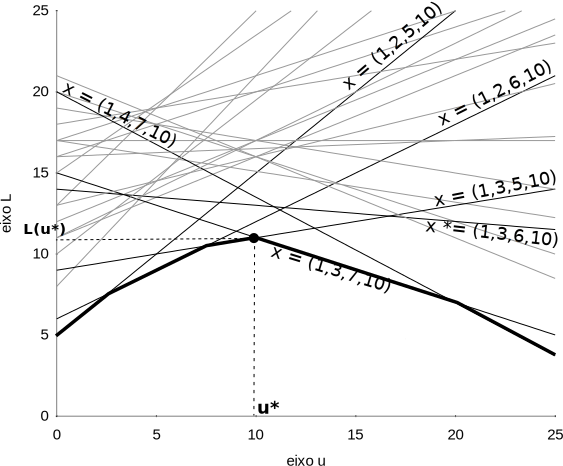
\includegraphics[scale=0.58]{figuras/exemplo_funcao_L.png}
%    \caption{\it Representa��o geom�trica do grafo da Figura \ref{fig:exemplo_grafo}.
%        As retas pretas represetam os caminhos que s�o relevantes ao algoritmo. A ``curva'' de segmentos
%    mais espessos representa o fun��o $L(u)$. }
%    \label{fig:exemplo_funcao_L}
%\end{figure}

%\end{frame}

\begin{frame}
    \frametitle{Relaxa��o Lagrangeana - Exemplo}
    \begin{figure}[h!]
        \centering
            \includegraphics[scale=0.31]{figuras/graph.pdf}
            \includegraphics[scale=0.31]{figuras/lines.pdf}
    \end{figure}
\end{frame}
\begin{frame}
    \frametitle{Relaxa��o Lagrangeana - Exemplo}
    \begin{figure}[h!]
        \centering
            \includegraphics[scale=0.31]{figuras/graph1.pdf}
            \includegraphics[scale=0.31]{figuras/lines1.pdf}
    \end{figure}
\end{frame}
\begin{frame}
    \frametitle{Relaxa��o Lagrangeana - Exemplo}
    \begin{figure}[h!]
        \centering
            \includegraphics[scale=0.31]{figuras/graph2.pdf}
            \includegraphics[scale=0.31]{figuras/lines2.pdf}
    \end{figure}
\end{frame}
\begin{frame}
    \frametitle{Relaxa��o Lagrangeana - Exemplo}
    \begin{figure}[h!]
        \centering
            \includegraphics[scale=0.31]{figuras/graph4.pdf}
            \includegraphics[scale=0.31]{figuras/lines4.pdf}
    \end{figure}
\end{frame}
\begin{frame}
    \frametitle{Relaxa��o Lagrangeana - Exemplo}
    \begin{figure}[h!]
        \centering
            \includegraphics[scale=0.31]{figuras/graph5.pdf}
            \includegraphics[scale=0.31]{figuras/lines5.pdf}
    \end{figure}
\end{frame}
\begin{frame}
    \frametitle{Relaxa��o Lagrangeana - Exemplo}
    \begin{figure}[h!]
        \centering
            \includegraphics[scale=0.31]{figuras/graph7.pdf}
            \includegraphics[scale=0.31]{figuras/lines7.pdf}
    \end{figure}
\end{frame}
\begin{frame}
    \frametitle{Relaxa��o Lagrangeana - Exemplo}
    \begin{figure}[h!]
        \centering
            \includegraphics[scale=0.31]{figuras/graph8.pdf}
            \includegraphics[scale=0.31]{figuras/lines8.pdf}
    \end{figure}
\end{frame}
\begin{frame}
    \frametitle{Relaxa��o Lagrangeana - Exemplo}
    \begin{figure}[h!]
        \centering
            \includegraphics[scale=0.31]{figuras/graph9.pdf}
            \includegraphics[scale=0.31]{figuras/lines9.pdf}
    \end{figure}
\end{frame}
\begin{frame}
    \frametitle{Relaxa��o Lagrangeana - Exemplo}
    \begin{figure}[h!]
        \centering
            \includegraphics[scale=0.31]{figuras/graph10.pdf}
            \includegraphics[scale=0.31]{figuras/lines10.pdf}
    \end{figure}
\end{frame}
\begin{frame}
    \frametitle{Relaxa��o Lagrangeana - Exemplo}
    \begin{figure}[h!]
        \centering
            \includegraphics[scale=0.31]{figuras/graph11.pdf}
            \includegraphics[scale=0.31]{figuras/lines11.pdf}
    \end{figure}
\end{frame}


%\section{Algoritmos de aproxima��o}

%\subsection{Um \fptas\ para o problema \rcsp}




% Copyright 2007 by Till Tantau
%
% This file may be distributed and/or modified
%
% 1. under the LaTeX Project Public License and/or
% 2. under the GNU Public License.
%
% See the file doc/licenses/LICENSE for more details.



\documentclass{beamer}

%
% DO NOT USE THIS FILE AS A TEMPLATE FOR YOUR OWN TALKS�!!
%
% Use a file in the directory solutions instead.
% They are much better suited.
%


% Setup appearance:

\usetheme{Darmstadt}
\usefonttheme[onlylarge]{structurebold}
\setbeamerfont*{frametitle}{size=\normalsize,series=\bfseries}
\setbeamertemplate{navigation symbols}{}


% Standard packages

\usepackage[portuguese]{babel}
\usepackage[latin1]{inputenc}
\usepackage{times}
\usepackage[T1]{fontenc}

%% definicao personalizada
\usepackage{../estilo/estilo}
%\usepackage{../estilo/tkz-graph}
%\usepackage{../estilo/tkz-berge}


% Setup TikZ

\usepackage{tikz}
\usetikzlibrary{arrows,petri,trees}
\tikzstyle{block}=[dra opacity=0.7,line width=1.4cm]


% Author, Title, etc.

\title[$k$-caminhos m�nimos] 
{%
  Exame de Qualifica��o \\
  $k$-caminhos m�nimos%
}
\author{F�bio Pisaruk}
\institute[IME/USP]
{%
Instituto de Matem�tica e Estat�stica \\
Universidade de S�o Paulo%
}
\date{\today}

\pgfdeclareimage[height=0.5cm]{ime-logo}{../figs/ime-arquimedes}
\pgfdeclareimage[height=4cm]{interligacao}{../figs/interligacao}
\pgfdeclareimage[height=3cm]{aprovisionamento}{../figs/aprovisionamento}
\pgfdeclareimage[height=3cm]{aprovisionamento2}{../figs/aprovisionamento2}
\pgfdeclareimage[height=3cm]{algoritmoAntigo}{../figs/algoritmoAntigo}
\pgfdeclareimage[height=5cm]{prefixo}{../figs/prefixo}

\logo{\pgfuseimage{ime-logo}}

% The main document

\begin{document}

\begin{frame}
  \titlepage
\end{frame}

\begin{frame}{Sum�rio}
   Este trabalho trata de algoritmos para gera��o de $k$-caminhos m�nimos sem circuitos em grafos n�o-dirigidos.
  \tableofcontents
\end{frame}


\section{Introdu��o}

\subsection{Problema}

\begin{frame}{Aprovisionamento de sinais}
	\begin{itemize}
		\item Servi�o de interliga��o de sinais.
		\item Permite que sinais do ponto $a$ sejam enviados ao ponto $b$.
	\end{itemize}
	\begin{figure}
	\pgfuseimage{interligacao}
   	\caption{Destacamos um poss�vel caminho interligando $a$ e $b$.}
	\end{figure}
\end{frame}

\begin{frame}{Processo de aprovisionamento}
 \begin{block}{Requisitos do cliente}
	\begin{itemize}
		\item Quantidade de sinais a serem interligados.
		\item Tipos de sinais.
		\item Origem e destino.
		\item Qualidade de servi�o.
	\end{itemize}
 \end{block}
\begin{figure}
	\pgfuseimage{aprovisionamento}
   	%\caption{Caminho entre $a$ e $b$ com cada elemento exibindo as quantidades usada e a m�xima de transmiss�o.}
	\end{figure}
\end{frame}

\begin{frame}{Processo de aprovisionamento}
\begin{block}{Considera��es}
	\begin{itemize}
		\item Custo � fun��o do n�mero de equipamentos usados.
		\item $k$ depende da quantidade de sinais.
		\item Crit�rio de desempate � a dist�ncia total.
	\end{itemize}
\end{block}
\begin{figure}
\pgfuseimage{aprovisionamento2}
%\caption{Caminho entre $a$ e $b$ com cada elemento exibindo as quantidades usada e a m�xima de transmiss�o.}
\end{figure}
\end{frame}


\subsection{Solu��es}

\begin{frame}{Algoritmo existente na empresa}
\framesubtitle{Busca exaustiva}
	\begin{figure}
	\pgfuseimage{algoritmoAntigo}
	\end{figure}
	\begin{columns}[t]
	  \begin{column}{2cm}
	    \onslide<1->
		{%
		\small{$\seq{a,b}$\\$\seq{a,c}$\\$\seq{a,d}$}
		}
	  \end{column}
	  \begin{column}{2cm}
	    \onslide<2->
	    {%
	    \small{$\seq{a,b,c}$\\\textcolor{red}{$\seq{a,b,e}$}\\$\seq{a,c,b}$\\\textcolor{red}{$\seq{a,c,e}$}\\$\seq{a,c,d}$\\$\seq{a,d,c}$\\\textcolor{red}{$\seq{a,d,e}$}}
	    }
	  \end{column}
          \begin{column}{2cm}
	    \onslide<3->
	    {%
	    \small{\textcolor{red}{$\seq{a,b,c,e}$}\\$\seq{a,b,c,d}$\\\textcolor{red}{$\seq{a,c,b,e}$}\\\textcolor{red}{$\seq{a,c,d,e}$}\\\textcolor{red}{$\seq{a,d,c,e}$}\\$\seq{a,d,c,b}$}
            }
	  \end{column}
          \begin{column}{2cm}
	 \onslide<4->
	    {%
	    \small{\textcolor{red}{$\seq{a,b,c,d,e}$}\\\textcolor{red}{$\seq{a,d,c,b,e}$}}
	    }
	  \end{column}
	\end{columns}
	\onslide<5->
	{%	
	\alert{Consumo elevado de mem�ria}.
	}
\end{frame}

\begin{frame}{Primeiro algoritmo implementado}
\framesubtitle{Busca em profundidade iterativa}
	\begin{figure}
	\pgfuseimage{algoritmoAntigo}
	\end{figure}
	\begin{columns}[t]
	  \begin{column}{2cm}
		\onslide<1->
		{%
		\begin{block}{n�vel 1}
		\end{block}
		}
	  \end{column}
	  \begin{column}{2cm}
		\onslide<2->
		{%
   	    \begin{block}{n�vel 2}
		 \textcolor{red}{$\seq{a,b,e}$}\\\textcolor{red}{$\seq{a,c,e}$}\\\textcolor{red}{$\seq{a,d,e}$}
	    \end{block}
		}
	  \end{column}
          \begin{column}{2cm}
	\onslide<3->
		{%
		\begin{block}{n�vel 3}
    	\textcolor{red}{$\seq{a,b,c,e}$}\\\textcolor{red}{$\seq{a,c,b,e}$}\\\textcolor{red}{$\seq{a,c,d,e}$}\\\textcolor{red}{$\seq{a,d,c,e}$}
	        \end{block}
		}
	  \end{column}
     \begin{column}{2cm}
	\onslide<4->
		{%
           \begin{block}{n�vel 4}
           \textcolor{red}{$\seq{a,b,c,d,e}$}\\\textcolor{red}{$\seq{a,d,c,b,e}$}
           \end{block}
		}
          \end{column}
      	\end{columns}
	\onslide<5->
	{%		
	\alert{Menor consumo de mem�ria e maior consumo de processador}.
	}
\end{frame}

\begin{frame}{Algoritmo final entregue}
\framesubtitle{Algoritmo de Katoh, Ibaraki e Mine(KIM)}
  \begin{tikzpicture}[scale=0.85]
    \tikzstyle{node}=%
    [%
      inner sep=0pt,%
      outer sep=0pt,%
      ball color=example text.fg,%
      circle%
    ]
        \node[node,minimum size=8pt,label=left:{s}] at (0,3) (S)  {};
        \node[node] at (1,3) (A)  {};
        \node[node] at (2,3) (B)  {};
        \node[node] at (3,3) (C)  {};
        \node[node] at (4,1) (D)  {};
        \node[node,minimum size=8pt,label=right:{t}] at (11,3) (T) {};
       
        \node[color=red] at (6,3.2) (P1) {P1};

        \path [-,thick,red]  
                  (S) edge[] (T)
                  (S) edge (A)
                  (A) edge (B)
                  (B) edge (C);
       \onslide<2->{
        \path [-,thick,blue]  
                  (B) edge[bend right] (D)
                  (D) edge[bend right] (T);
         \node[color=blue] at (6,1) (P2) {P2};

        }
        \onslide<5->{
        \path [-,thick,black,dashed]  
                  (A.north) edge[in=90] (T.north);
                 \node[color=black] at (6,5.8) (Pc) {Pc};
}
        \onslide<3->{
        \path [-,thick,black,dashed]  
                  (C.north) edge[bend left] (T.north);
                 \node[color=black] at (6,4.5) (Pa) {Pa};
}
       \onslide<4->{
        \path [-,thick,black,dashed]  
                  (D) edge[in=-90,out=-90] (T);
                 \node[color=black] at (6,0) (Pb) {Pb};
}
        \end{tikzpicture}
        
        
        %\begin{figure}
	%\pgfuseimage{kimCaminhos}
	%\caption{\\
	%	$P1$ : caminho m�nimo entre $s$ e $t$. \\
%		$P2$ : caminho m�nimo diferente de $P1$. \\ 
%		$Pa$,$Pb$,$Pc$: caminhos candidatos.}	
%	\end{figure}
\end{frame}

\section{k-caminhos m�nimos}
\subsection{Defini��o}
\begin{frame}{Problema $k$-caminhos m�nimos}
 \begin{quote}
   \textbf{Problema} \kCM$(V,A,c,s,t,k)$:
	\begin{itemize}   
	\item Grafo: $(V,A)$
	\item Fun��o custo: $c$
	\item V�rtices: $s$ e $t$ 
	\item Inteiro positivo: $k$ 
	\end{itemize}	
	
	
	Encontrar $k$-caminhos de custos m�nimos 
	de $s$ a $t$.
 \end{quote}
\end{frame}

\begin{frame}{M�todo gen�rico}
\begin{algoritmo}

\textbf{M�todo} \Generico{} $(V,A,c,s,t,k)$ %\\[2mm]
   
0\x $\Pcal \larr \mbox{conjunto dos caminhos de $s$ a~$t$}$ 

1\x \para{} $i=1,\ldots,k$ \faca %\\[1mm]

2\xx  $P_i \larr \mbox{caminho de custo m�nimo em $\Pcal$}$ %\\[1mm]

3\xx  $\Pcal \larr \Pcal - P_i$

4\x \devolva{} $\seq{P_1,\ldots,P_k}$

\end{algoritmo}

\end{frame}

\begin{frame}{Exemplo}
  \begin{columns}
    \column{.7\textwidth}
  \begin{tikzpicture}[auto,thick,sloped,node distance=18mm]
    \tikzstyle{every node}=%
    [%
      minimum size=12pt,%
      inner sep=0pt,%
      outer sep=0pt,%
      ball color=example text.fg,%
      circle%
    ]
        \node[ball color=red] (S) {s};
        \node (B) [right of=S] {b};
        \node (G) [right of=B] {g};
        \node (L) [right of=G] {l};
        \node[ball color=red] (T) [right of=L] {t};
        \node (F) [above of=G] {f};
        \node (E) [above of=F] {e};
        \node (H) [below of=G] {h};
        \node (I) [below of=H] {i};
        \node (C) [above of=S] {c};
        \node (A) [below of=S] {a};
        \node (J) [above of=L] {j};
        \node (D) [left of=E] {d};

          
          \path [-,thick,black] (S) edge (A)
                                    edge (B)
                                    edge (C)
                                (B) edge (C)
                                    edge (D)
                                    edge (F)
                                    edge (G)
                                    edge (H)
                                (D) edge (E)   
                                (A) edge (I)
                                (I) edge (H)
                                    edge (T)
                                (E) edge (F)
                                    edge (J)
                                (F) edge (G)
                                (F) edge (L)
                                (G) edge (H)
                                    edge (L)  
                                (J) edge (L)
                                (L) edge (T)
                                (H) edge (L)
                                (C) edge (D);

          \uncover<2>{
          \path[-,thick,red,line width=1mm] (S) edge (A)
                            (A) edge (I)
                            (I) edge (T);
          }
          \uncover<3>{
          \path[-,thick,red,line width=1mm] (S) edge (B)
                            (B) edge (F)
                            (F) edge (L)
                            (L) edge (T) ;
          }
          \uncover<4>{
          \path[-,thick,red,line width=1mm] (S) edge (B)
                            (B) edge (G)
                            (G) edge (L)
                            (L) edge (T) ;
          }
          \uncover<5>{
          \path[-,thick,red,line width=1mm] (S) edge (B)
                            (B) edge (H)
                            (H) edge (L)
                            (L) edge (T) ;
          }
          \uncover<6>{
          \path[-,thick,red,line width=1mm] (S) edge (B)
                            (B) edge (H)
                            (H) edge (I)
                            (I) edge (T) ;
          }
          \uncover<7>{
          \path[-,thick,red,line width=1mm] (S) edge (A)
                            (A) edge (I)
                            (I) edge (H)
                            (H) edge (L)
                            (L) edge (T);
          }
  \end{tikzpicture}

    \column{.3\textwidth}
   \begin{block}{Caminhos}
      \onslide<2->{$\seq{s,a,i,t}$} \\
      \onslide<3->{$\seq{s,b,f,l,t}$} \\
      \onslide<4->{$\seq{s,b,g,l,t}$} \\
      \onslide<5->{$\seq{s,b,h,l,t}$} \\
      \onslide<6->{$\seq{s,b,h,i,t}$} \\
      \onslide<7->{$\seq{s,a,i,h,l,t}$}
 \end{block}

  \end{columns}  

\end{frame}

%\begin{frame}{Exemplo}
%	\only<1>
%	{%
%	\begin{figure}
%	\pgfuseimage{grafoExemplo1}
%	\caption{6-caminhos m�nimos}
%	\end{figure}
%	}
%	\only<2>
%	{%
%	\begin{figure}
%	\pgfuseimage{grafoExemplo2}
%	\caption{	$\seq{s,a,i,t}$
%		}
%	\end{figure}
%	}
%	\only<3>
%	{%
%	\begin{figure}
%	\pgfuseimage{grafoExemplo3}
%	\caption{	$\seq{s,a,i,t}$,
%			$\seq{s,b,f,l,t}$
%		}
%	\end{figure}
%	}
%	\only<4>
%	{%
%	\begin{figure}
%	\pgfuseimage{grafoExemplo4}
%	\caption{	$\seq{s,a,i,t}$,
%			$\seq{s,b,f,l,t}$,
%			$\seq{s,b,g,l,t}$
%		}
%	\end{figure}
%	}
%	\only<5>
%	{%
%	\begin{figure}
%	\pgfuseimage{grafoExemplo5}
%	\caption{	$\seq{s,a,i,t}$,
%			$\seq{s,b,f,l,t}$,
%			$\seq{s,b,g,l,t}$,
%			$\seq{s,b,h,l,t}$
%	}
%	\end{figure}
%	}
%	\only<6>
%	{%
%	\begin{figure}
%	\pgfuseimage{grafoExemplo6}
%	\caption{	$\seq{s,a,i,t}$,
%			$\seq{s,b,f,l,t}$,
%			$\seq{s,b,g,l,t}$,
%			$\seq{s,b,h,l,t}$,
%			$\seq{s,b,h,i,t}$
%	}
%	\end{figure}
%	}
%	\only<7>
%	{%
%	\begin{figure}
%	\pgfuseimage{grafoExemplo7}
%	\caption{	$\seq{s,a,i,t}$,
%			$\seq{s,b,f,l,t}$,
%			$\seq{s,b,g,l,t}$,
%			$\seq{s,b,h,l,t}$,
%			$\seq{s,b,h,i,t}$,
%			$\seq{s,a,i,h,l,t}$
%	}
%	\end{figure}
%	}
%
%\end{frame}

\begin{frame}{Exemplo: �rvore de caminhos}
	$\seq{s,a,i,t}$,
	$\seq{s,b,f,l,t}$,
	$\seq{s,b,g,l,t}$,
	$\seq{s,b,h,l,t}$,
	$\seq{s,b,h,i,t}$,
	$\seq{s,a,i,h,l,t}$
\begin{center}
\begin{tikzpicture}[auto,thick,sloped]
  \tikzstyle{node}=%
  [%
    minimum size=8pt,%
    inner sep=0pt,%
    outer sep=0pt,%
    ball color=example text.fg,%
    circle%
  ]
  \tikzstyle{leaf}=%
  [%
    minimum size=10pt,%
    inner sep=0pt,%
    outer sep=0pt,%
    ball color=red,%
    circle%
  ]

% Set the overall layout of the tree
\tikzstyle{level 1}=[level distance=1cm, sibling distance=5cm]
\tikzstyle{level 2}=[level distance=1cm, sibling distance=2cm]

% Define styles for bags and leafs
\tikzstyle{bag} = [text width=4em, text centered]
\tikzstyle{end} = [circle, minimum width=3pt,fill, inner sep=0pt]
  \node [leaf,label=above:{s}] {} [->] 
    child {
	node [node,label=above:{a}] {} 
	child {
		node [node,label=right:{i}] {} 
		child 	{
				node [leaf,label=below:{t1}] {} 	
				edge from parent 
			}
		child 	{
				node [node,label=right:{h}] {} 
				child {
					node [node,label=right:{l}] {} 
					child{
						node [leaf,label=below:{t6}] {} 
						edge from parent 
					}
					edge from parent 
				}
				edge from parent 
			}
		edge from parent 
		}
	edge from parent 
        }	
	child {
		node [node,label=above:{b}] {} 	
   		child {
			node [node,label=above:{f}] {} 	
   			child {
				node [node,label=left:{l}] {} 
				child{
					node [leaf,label=below:{t2}] {} 
					edge from parent 
				}
				edge from parent 
			}
			edge from parent 
		}	
	  	child {
			node [node,label=left:{g}] {} 	
   			child {
				node [node,label=left:{l}] {} 
				child{
					node [leaf,label=below:{t3}] {} 
					edge from parent
				}
				edge from parent 
			}
			edge from parent 
		}		
	  	child {
			node [node,label=above:{h}] {} 	
   			child {
				node [node,label=above:{l}] {} 
				child{
					node [leaf,label=below:{t4}] {} 
					edge from parent
				}
				edge from parent 
			}
   			child {
				node [node,label=above:{i}] {} 
				child{
					node [leaf,label=below:{t5}] {} 
					edge from parent 
				}
				edge from parent 
			}
			edge from parent 
		}	
		edge from parent 
	};
\end{tikzpicture}
\end{center}
\end{frame}


\subsection{�rvore dos prefixos}
\begin{frame}{Defini��o}
\framesubtitle{\textbf{$\Qcal,(N,E),f,V(\Qcal),A(\Qcal)$}}
\begin{itemize}
	\only<1>{
        \item $\Qcal$: uma cole��o de caminhos
        \begin{columns}
          \column{.3\textwidth}
        \begin{block}{Caminhos}
            {$\seq{s,a,i,t}$} \\
            {$\seq{s,b,f,l,t}$} \\
            {$\seq{s,b,g,l,t}$} \\
            {$\seq{s,b,h,l,t}$} \\
            {$\seq{s,b,h,i,t}$} \\
            {$\seq{s,a,i,h,l,t}$}
        \end{block}
        \end{columns}
        \mbox{} \\
        \mbox{} \\
        \mbox{} \\
     }
	\only<2>{
        \item $(N,E)$: uma arboresc�ncia
        \begin{center}
        \begin{tikzpicture}[auto,thick]
          \tikzstyle{node}=%
          [%
            minimum size=10pt,%
            inner sep=0pt,%
            outer sep=0pt,%
            ball color=example text.fg,%
            circle%
          ]

          \node [node] {A} [->]
            child {node [node] {B} edge from parent node[swap]{a}}
            child {node [node] {E} edge from parent node{e}}
            child {node [node] {C} 
                child {node [node] {D} edge from parent node{c}}
                edge from parent node{b}
            };
        \end{tikzpicture}
        \end{center}
        \begin{itemize}
        \item Grafo ac�clico $(N,E)$ 
        \item $|N| = |E| + 1$ 
        \item \defi{raiz}
        \end{itemize}
        Todo v�rtice, exceto a \defi{raiz}, � ponta final de exatamente um arco.
        }
	\only<3>{
        \item $f$: uma \defi{fun��o r�tulo} 
  \begin{block}{}
	\textbf{Associa n�s e arestas do grafo aos n�s e arestas da �rvore de prefixos.}
  \end{block}
  Se \begin{eqnarray*}
  R=\seq{u_{0}, e_{1}, u_{1}, \ldots, e_{t}, u_{t}}
  \end{eqnarray*}
  for um caminho em  $(N,E)$, ent�o
  \begin{eqnarray*}
  f(R):=\seq{f(u_{0}), f(e_{1}), f(u_{1}), \ldots, f(e_{t}), f(u_{t})}
  \end{eqnarray*}
  ser� uma seq��ncia de v�rtices e arcos dos caminhos em $\Qcal$.
        \mbox{} \\
        \mbox{} \\
        \mbox{} \\
        \mbox{} \\
        \mbox{} \\
        }
        \only<1>{
	\item $V(\Qcal)$: conjunto de v�rtices
	\item $A(\Qcal)$: conjunto de arcos
        }
\end{itemize}
\end{frame}

%Seja $(N,E)$ uma arboresc�ncia e  
%$f$ uma \defi{fun��o r�tulo} que associa a cada n� em 
%$N$ um v�rtice em $V(\Qcal)$ e a
%cada arco em $E$ um arco em $A(\Qcal)$. 

%\begin{frame}{Defini��o}
%$(N,E,f)$ � \defi{�rvore dos prefixos} de $\Qcal$ se 
%\begin{itemize}
%\item para cada caminho $R$ em $(N,E)$ com in�cio na
%      raiz, $f(R)$ for prefixo de algum caminho em $\Qcal$; e
%\item para cada prefixo $Q$ de algum caminho em $\Qcal$
%      existir um caminho $R$ em $(N,E)$ com in�cio na
%      raiz tal que $f(R)=Q$; e
%\item o caminho $R$ do item anterior for �nico. 
%\end{itemize}
%\end{frame}

\begin{frame}{Exemplo}
  \begin{columns}  
    \column{.4\textwidth}
  \begin{tikzpicture}[auto,thick,sloped,node distance=9mm,scale=0.7]
    \tikzstyle{every node}=%
    [%
      inner sep=0pt,%
      outer sep=0pt,%
      ball color=example text.fg,%
      circle%
    ]
        \node[ball color=red] (S) {s};
        \node (B) [right of=S] {b};
        \node (G) [right of=B] {g};
        \node (L) [right of=G] {l};
        \node[ball color=red] (T) [right of=L] {t};
        \node (F) [above of=G] {f};
        \node (E) [above of=F] {e};
        \node (H) [below of=G] {h};
        \node (I) [below of=H] {i};
        \node (C) [above of=S] {c};
        \node (A) [below of=S] {a};
        \node (J) [above of=L] {j};
        \node (D) [left of=E] {d};

          
          \path [-,thick,black] (S) edge (A)
                                    edge (B)
                                    edge (C)
                                (B) edge (C)
                                    edge (D)
                                    edge (F)
                                    edge (G)
                                    edge (H)
                                (D) edge (E)   
                                (A) edge (I)
                                (I) edge (H)
                                    edge (T)
                                (E) edge (F)
                                    edge (J)
                                (F) edge (G)
                                (F) edge (L)
                                (G) edge (H)
                                    edge (L)  
                                (J) edge (L)
                                (L) edge (T)
                                (H) edge (L)
                                (C) edge (D);

          \uncover<2>{
          \path[-,thick,red,line width=1mm] (S) edge (A)
                            (A) edge (I)
                            (I) edge (T);
          }
          \uncover<3>{
          \path[-,thick,red,line width=1mm] (S) edge (B)
                            (B) edge (F)
                            (F) edge (L)
                            (L) edge (T) ;
          }
          \uncover<4>{
          \path[-,thick,red,line width=1mm] (S) edge (B)
                            (B) edge (G)
                            (G) edge (L)
                            (L) edge (T) ;
          }
          \uncover<5>{
          \path[-,thick,red,line width=1mm] (S) edge (B)
                            (B) edge (H)
                            (H) edge (L)
                            (L) edge (T) ;
          }
          \uncover<6>{
          \path[-,thick,red,line width=1mm] (S) edge (B)
                            (B) edge (H)
                            (H) edge (I)
                            (I) edge (T) ;
          }
          \uncover<7>{
          \path[-,thick,red,line width=1mm] (S) edge (A)
                            (A) edge (I)
                            (I) edge (H)
                            (H) edge (L)
                            (L) edge (T);
          }
  \end{tikzpicture}

    \column{.6\textwidth}
\begin{tikzpicture}[auto,thick,sloped,scale=0.7]
  \tikzstyle{node}=%
  [%
    minimum size=8pt,%
    inner sep=0pt,%
    outer sep=0pt,%
    ball color=example text.fg,%
    circle%
  ]
  \tikzstyle{leaf}=%
  [%
    minimum size=10pt,%
    inner sep=0pt,%
    outer sep=0pt,%
    ball color=red,%
    circle%
  ]

% Set the overall layout of the tree
\tikzstyle{level 1}=[level distance=1cm, sibling distance=5cm]
\tikzstyle{level 2}=[level distance=1cm, sibling distance=2cm]

% Define styles for bags and leafs
\tikzstyle{bag} = [text width=4em, text centered]
\tikzstyle{end} = [circle, minimum width=3pt,fill, inner sep=0pt]
\uncover<2>{
  \node [leaf,label=above:{s}] (raiz){} [] 
    child {
	node [node,label=right:{a}] (sa) {} 
  	child {
		node [node,label=right:{i}] (sai) {} 
		child 	{
				node [leaf,label=below:{t1}] (sait){} 	
				edge from parent 
			}
		edge from parent 
	}
	edge from parent
   };
	\path[opacity=1,color=red,->] [-latex]
	(raiz) edge (sa)
	(sa) edge (sai)
	(sai) edge (sait);
}
\uncover<3>{
  \node [leaf,label=above:{s}] (raiz) {} [] 
    	child {
		node [node,label=above:{a}] {} [->]
		child {
			node [node,label=right:{i}] {} [->]
			child 	{
					node [leaf,label=below:{t1}] {} [->]	
					edge from parent 
				}
			edge from parent 
			}
		edge from parent 
        }	
	child {
		node [node,label=above:{b}] (sb){} 	
   		child {
			node [node,label=left:{f}] (sbf) {} 	
   			child {
				node [node,label=left:{l}] (sbfl) {} 
				child{
					node [leaf,label=below:{t2}] (sbflt) {} 
					edge from parent 
				}
				edge from parent 
			}
			edge from parent 
		}	
		edge from parent 
	};
	\path[opacity=1,color=red,->] [-latex]
	(raiz) edge (sb)
	(sb) edge (sbf)
	(sbf) edge (sbfl)
	(sbfl) edge (sbflt);
}
\uncover<4>{
  \node [leaf,label=above:{s}] (raiz) {} [] 
    child {
	node [node,label=above:{a}] {} [->]
	child {
		node [node,label=right:{i}] {} [->]
		child 	{
				node [leaf,label=below:{t1}] {} [->]	
				edge from parent 
			}
		edge from parent 
		}
	edge from parent 
        }	
	child {
		node [node,label=above:{b}] (sb) {} []	
   		child {
			node [node,label=above:{f}]  {} [->] 	
   			child {
				node [node,label=left:{l}] {} [->]
				child{
					node [leaf,label=below:{t2}] {} [->]
					edge from parent 
				}
				edge from parent 
			}
			edge from parent 
		}	
	  	child {
			node [node,label=left:{g}] (sbg){} 	
   			child {
				node [node,label=left:{l}] (sbgl) {} 
				child{
					node [leaf,label=below:{t3}] (sbglt) {} 
					edge from parent
				}
				edge from parent 
			}
			edge from parent 
		}		
		edge from parent 
	};
	\path[opacity=1,color=red,->] [-latex]
	(raiz) edge (sb)
	(sb) edge (sbg)
	(sbg) edge (sbgl)
	(sbgl) edge (sbglt);
}
\uncover<5>{
  \node [leaf,label=above:{s}] (raiz) {} [] 
    child {
	node [node,label=above:{a}] {} [->]
	child {
		node [node,label=right:{i}] {}  
		child 	{
				node [leaf,label=below:{t1}] {} 	
				edge from parent 
			}
		edge from parent 
		}
	edge from parent 
        }	
	child {
		node [node,label=above:{b}] (sb) {} 	
   		child {
			node [node,label=above:{f}] {} 	[->]
   			child {
				node [node,label=left:{l}] {} 
				child{
					node [leaf,label=below:{t2}] {} 
					edge from parent 
				}
				edge from parent 
			}
			edge from parent 
		}	
	  	child {
			node [node,label=left:{g}] {} [->]	
   			child {
				node [node,label=left:{l}] {} 
				child{
					node [leaf,label=below:{t3}] {} 
					edge from parent
				}
				edge from parent 
			}
			edge from parent 
		}		
	  	child {
			node [node,label=right:{h}] (sbh) {} 	
   			child {
				node [node,label=right:{l}] (sbhl) {} 
				child{
					node [leaf,label=below:{t4}] (sbhlt) {} 
					edge from parent
				}
				edge from parent 
			}
			edge from parent 
		}	
		edge from parent 
	};
	\path[opacity=1,color=red,->] [-latex]
	(raiz) edge (sb)
	(sb) edge (sbh)
	(sbh) edge (sbhl)
	(sbhl) edge (sbhlt);

}
\uncover<6>{
  \node [leaf,label=above:{s}] (raiz) {} [] 
    child {
	node [node,label=above:{a}] {} [->]
	child {
		node [node,label=right:{i}] {} 
		child 	{
				node [leaf,label=below:{t1}] {} 	
				edge from parent 
			}
		edge from parent 
		}
	edge from parent 
        }	
	child {
		node [node,label=above:{b}] (sb){} 	
   		child {
			node [node,label=above:{f}] {} 	[->]
   			child {
				node [node,label=left:{l}] {} 
				child{
					node [leaf,label=below:{t2}] {} 
					edge from parent 
				}
				edge from parent 
			}
			edge from parent 
		}	
	  	child {
			node [node,label=left:{g}] {} 	[->]
   			child {
				node [node,label=left:{l}] {} 
				child{
					node [leaf,label=below:{t3}] {} 
					edge from parent
				}
				edge from parent 
			}
			edge from parent 
		}		
	  	child {
			node [node,label=above:{h}] (sbh){} 	
   			child {
				node [node,label=above:{l}] {} [->]
				child{
					node [leaf,label=below:{t4}] {} 
					edge from parent
				}
				edge from parent 
			}
   			child {
				node [node,label=above:{i}] (sbhi){} 
				child{
					node [leaf,label=below:{t5}] (sbhit) {} 
					edge from parent 
				}
				edge from parent 
			}
			edge from parent 
		}	
		edge from parent 
	};
	\path[opacity=1,color=red,->] [-latex]
	(raiz) edge (sb)
	(sb) edge (sbh)
	(sbh) edge (sbhi)
	(sbhi) edge (sbhit);
}
\uncover<7>{
  \node [leaf,label=above:{s}] (raiz) {} [] 
    child {
	node [node,label=above:{a}] (sa) {} 
	child {
		node [node,label=right:{i}] (sai){} 
		child 	{
				node [leaf,label=below:{t1}] {} [->]	
				edge from parent 
			}
		child 	{
				node [node,label=right:{h}] (saih){} 
				child {
					node [node,label=right:{l}](saihl) {} 
					child{
						node [leaf,label=below:{t6}] (saihlt) {} 
						edge from parent 
					}
					edge from parent 
				}
				edge from parent 
			}
		edge from parent 
		}
	edge from parent 
        }	
	child {
		node [node,label=above:{b}] {} [->]	
   		child {
			node [node,label=above:{f}] {} 	
   			child {
				node [node,label=left:{l}] {} 
				child{
					node [leaf,label=below:{t2}] {} 
					edge from parent 
				}
				edge from parent 
			}
			edge from parent 
		}	
	  	child {
			node [node,label=left:{g}] {} [->]	
   			child {
				node [node,label=left:{l}] {} 
				child{
					node [leaf,label=below:{t3}] {} 
					edge from parent
				}
				edge from parent 
			}
			edge from parent 
		}		
	  	child {
			node [node,label=above:{h}] {} [->]
   			child {
				node [node,label=above:{l}] {} 
				child{
					node [leaf,label=below:{t4}] {} 
					edge from parent
				}
				edge from parent 
			}
   			child {
				node [node,label=above:{i}] {} 
				child{
					node [leaf,label=below:{t5}] {} 
					edge from parent 
				}
				edge from parent 
			}
			edge from parent 
		}	
		edge from parent 
	};
	\path[opacity=1,color=red,->] [-latex]
	(raiz) edge (sa)
	(sa) edge (sai)
	(sai) edge (saih)
	(saih) edge (saihl)	
	(saihl) edge (saihlt);
}
\end{tikzpicture}

  \end{columns}
\end{frame}

\subsection{M�todos}
\begin{frame}{M�todo \YenGenerico}
\begin{algoritmo}

\textbf{M�todo} \YenGenerico{} $(V,A,c,s,t,k)$ %\\[2mm]
   
0\x $\Pi \larr \{\{\mbox{conjunto dos caminhos de $s$ a~$t$}\}\}$

1\x $\Qcal \larr \emptyset $

2\x \para{} $i=1,\ldots,k$ \faca %\\[1mm]

3\xx  $\Lcal  \larr \seq{P_{\pi} : P_{\pi} \ \mbox{� caminho m�nimo da parte $\pi$
de~$\Pi$}}$

4\xx  $P_i \larr \mbox{caminho de custo m�nimo em $\Lcal$}$ %\\[1mm]

5\xx  $\Qcal \larr \Qcal \cup \{P_i\}$

6\xx  $\Pi \larr \AtualizeGenerico~(V,A,\Qcal)$

7\x \devolva{} $\seq{P_1,\ldots,P_k}$

\end{algoritmo}

\end{frame}

\begin{frame}{\AtualizeGenerico}

\begin{algoritmo}

\textbf{Algoritmo} \AtualizeGenerico{} $(V,A,\Qcal)$ %\\[2mm]
   
0\x $\Pi \larr \emptyset \quad \quad \Pcal \larr \Pcal_{st} \setminus \Qcal$

1\x $(N,E,f) \larr$ �rvore dos prefixos de $\Qcal$

2\x \para{} \cada{} $u \in N$ \faca %\\[1mm]

3\xx  $\pi_u \larr \{\mbox{caminhos em $\Pcal$ com prefixo $f(R_u)$}$

\xxxxx \quad e que n�o possuem arcos em $A_u \}$

4\xx  $\Pi \larr  \Pi \cup \{\pi_u\}$ %\\[1mm]

5\x \devolva{} $\Pi$

\end{algoritmo}
\end{frame}

\begin{frame}{Exemplo}
  \begin{columns}  
    \column{.4\textwidth}
  \begin{tikzpicture}[auto,thick,sloped,node distance=9mm,scale=0.7]
    \tikzstyle{every node}=%
    [%
      inner sep=0pt,%
      outer sep=0pt,%
      ball color=example text.fg,%
      circle%
    ]
        \node[ball color=red] (S) {s};
        \node (B) [right of=S] {b};
        \node (G) [right of=B] {g};
        \node (L) [right of=G] {l};
        \node[ball color=red] (T) [right of=L] {t};
        \node (F) [above of=G] {f};
        \node (E) [above of=F] {e};
        \node (H) [below of=G] {h};
        \node (I) [below of=H] {i};
        \node (C) [above of=S] {c};
        \node (A) [below of=S] {a};
        \node (J) [above of=L] {j};
        \node (D) [left of=E] {d};
          
         \path [-,thick,black] (S) edge (A)
                                    edge (B)
                                    edge (C)
                                (B) edge (C)
                                    edge (D)
                                    edge (F)
                                    edge (G)
                                    edge (H)
                                (D) edge (E)   
                                (A) edge (I)
                                (I) edge (H)
                                    edge (T)
                                (E) edge (F)
                                    edge (J)
                                (F) edge (G)
                                (F) edge (L)
                                (G) edge (H)
                                    edge (L)  
                                (J) edge (L)
                                (L) edge (T)
                                (H) edge (L)
                                (C) edge (D);
        \uncover<3>{  
	\path[-,thick,red,line width=1mm] (S) edge (B)
                            (B) edge (H)
                            (H) edge (L)
                            (L) edge (T) ;
	}
           \end{tikzpicture}

    \column{.6\textwidth}
\begin{tikzpicture}[auto,thick,sloped,scale=0.7]
  \tikzstyle{node}=%
  [%
    minimum size=8pt,%
    inner sep=0pt,%
    outer sep=0pt,%
    ball color=example text.fg,%
    circle%
  ]
  \tikzstyle{leaf}=%
  [%
    minimum size=10pt,%
    inner sep=0pt,%
    outer sep=0pt,%
    ball color=red,%
    circle%
  ]

% Set the overall layout of the tree
\tikzstyle{level 1}=[level distance=1.5cm, sibling distance=6cm]
\tikzstyle{level 2}=[level distance=2cm, sibling distance=2cm]

% Define styles for bags and leafs
\tikzstyle{bag} = [text width=4em, text centered]
\tikzstyle{end} = [circle, minimum width=3pt,fill, inner sep=0pt]
\only<1>{
 \node[draw,color=red] at (3.5,0) {$f(R_u) = \seq{s,b}$};
 \node[color=blue,rectangle,draw,dashed,opacity=.5,minimum width=10pt] at (2.5,-2.6)  (Au) 
          {$A_u$ \mbox{ }\mbox{ }\mbox{ }\mbox{ }\mbox{ }\mbox{ }\mbox{ }\mbox{ }\mbox{ }\mbox{ }\mbox{ }\mbox{ }\mbox{ }\mbox{ }\mbox{ }\mbox{ }\mbox{ }\mbox{ }\mbox{ }\mbox{ }\mbox{ }\mbox{ }\mbox{ }\mbox{ }\mbox{ }\mbox{ }\mbox{ }};
  \node [leaf,label=above:{s}] (raiz) {} [] 
    child {
	node [node,label=above:{a}] {} [->]
	child {
		node [node,label=right:{i}] {} 
		child 	{
				node [leaf,label=below:{t1}] {} 	
				edge from parent 
			}
		edge from parent 
		}
	edge from parent 
        }	
	child {
		node [node,label=right:{$u$=b}] (sb) {} 	
   		child {
			node [node,label=left:{f},ball color=blue](sbf) {} 	
   			child {
				node [node,label=left:{l}] {} [->]
				child{
					node [leaf,label=below:{t2}] {} 
					edge from parent 
				}
				edge from parent 
			}
			edge from parent 	
	        }	
	  	child {
			node [node,label=right:{g},ball color=blue] (sbg) {} 	
   			child {
				node [node,label=left:{l}] {} [->]
				child{
					node [leaf,label=below:{t3}] {} 
					edge from parent
				}
				edge from parent 
			}
			edge from parent 
		}		
		edge from parent
 	};
	\path[opacity=1,color=red,->] [-latex]
	(raiz) edge (sb);
	\path[opacity=1,color=blue,->] [-latex]
	(sb) edge (sbf);
	\path[opacity=1,color=blue,->] [-latex]
	(sb) edge (sbg);
}

\only<2>{
 \node[draw,color=red] at (3.5,0) {$f(R_u) = \seq{s,b}$};
% \node[color=blue,rectangle,draw,dashed,opacity=.5,minimum width=10pt] at (2.5,-2.2)  (Au) 
%          {$A_u$ \mbox{ }\mbox{ }\mbox{ }\mbox{ }\mbox{ }\mbox{ }\mbox{ }\mbox{ }\mbox{ }\mbox{ }\mbox{ }\mbox{ }\mbox{ }\mbox{ }\mbox{ }\mbox{ }\mbox{ }\mbox{ }\mbox{ }\mbox{ }\mbox{ }\mbox{ }\mbox{ }\mbox{ }\mbox{ }\mbox{ }\mbox{ }};
  \node [leaf,label=above:{s}] (raiz) {} [] 
    child {
	node [node,label=above:{a}] {} [->]
	child {
		node [node,label=right:{i}] {} 
		child 	{
				node [leaf,label=below:{t1}] {} 	
				edge from parent 
			}
		edge from parent 
		}
	edge from parent 
        }	
	child {
		node [node,label=right:{$u$=b}] (sb) {} 	
   		child  [sibling distance=1.5cm]{
			node [node,label=left:{f},ball color=blue](sbf) {} 	
   			child {
				node [node,label=left:{l}] {} [->]
				child{
					node [leaf,label=below:{t2}] {} 
					edge from parent 
				}
				edge from parent 
			}
			edge from parent 	
	        }	
	  	child  [sibling distance=1.5cm]{
			node [node,label=right:{g},ball color=blue] (sbg) {} 	
   			child {
				node [node,label=left:{l}] {} [->]
				child{
					node [leaf,label=below:{t3}] {} 
					edge from parent
				}
				edge from parent 
			}
			edge from parent 
		}		
		child [sibling distance=1.5cm]{
			node [node,label=right:{c},ball color=gray] (sbc) {} [] 
			child{
				node [node,ball color=gray] {\ldots} [->]	
				child{
					node [node,label=below:{t},ball color=red] {} []	
		  			edge from parent 
				}
   				edge from parent 
			}
   			edge from parent 
		}	
		child [sibling distance=1.5cm]{
			node [node,label=right:{d},ball color=gray] (sbd) {} []
			child{
				node [node,ball color=gray] {\ldots} [->]	
				child{
					node [node,label=below:{t},ball color=red] {} []	
		  			edge from parent 
				}
   				edge from parent 
			}
   			edge from parent 
		}	
		child [sibling distance=1.5cm]{
			node [node,label=right:{h},ball color=gray] (sbh) {} []
			child{
				node [node,ball color=gray] {\ldots} [->]	
				child{
					node [node,label=below:{t},ball color=red] {} []	
		  			edge from parent 
				}
   				edge from parent 
			}
   			edge from parent 
		}	
	edge from parent
 	};
	\path[opacity=1,color=red,->] [-latex]
	(raiz) edge (sb);
	\path[opacity=1,color=blue,->] [-latex]
	(sb) edge (sbf);
	\path[opacity=1,color=blue,->] [-latex]
	(sb) edge (sbg);
	\path[dashed,opacity=1,color=gray,->] [-latex]
	(sb) edge (sbc);
	\path[dashed,opacity=1,color=gray,->] [-latex]
	(sb) edge (sbd);
	\path[dashed,opacity=1,color=gray,->] [-latex]
	(sb) edge (sbh);
	\draw[opacity=0.2,dashed,color=gray,fill] (2.5,-8.5) rectangle (6.8,-2.3);	
	\node at (6.5,-2.5) {$\pi_u$};
}
\only<3>{
 \node[draw,color=red] at (3.5,0) {$f(R_u) = \seq{s,b}$};
% \node[color=blue,rectangle,draw,dashed,opacity=.5,minimum width=10pt] at (2.5,-2.2)  (Au) 
%          {$A_u$ \mbox{ }\mbox{ }\mbox{ }\mbox{ }\mbox{ }\mbox{ }\mbox{ }\mbox{ }\mbox{ }\mbox{ }\mbox{ }\mbox{ }\mbox{ }\mbox{ }\mbox{ }\mbox{ }\mbox{ }\mbox{ }\mbox{ }\mbox{ }\mbox{ }\mbox{ }\mbox{ }\mbox{ }\mbox{ }\mbox{ }\mbox{ }};
  \node [leaf,label=above:{s}] (raiz) {} [] 
    child {
	node [node,label=above:{a}] {} [->]
	child {
		node [node,label=right:{i}] {} 
		child 	{
				node [leaf,label=below:{t1}] {} 	
				edge from parent 
			}
		edge from parent 
		}
	edge from parent 
        }	
	child {
		node [node,label=right:{$u$=b}] (sb) {} 	
   		child  [sibling distance=1.5cm]{
			node [node,label=left:{f},ball color=blue](sbf) {} 	
   			child {
				node [node,label=left:{l}] {} [->]
				child{
					node [leaf,label=below:{t2}] {} 
					edge from parent 
				}
				edge from parent 
			}
			edge from parent 	
	        }	
	  	child  [sibling distance=1.5cm]{
			node [node,label=right:{g},ball color=blue] (sbg) {} 	
   			child {
				node [node,label=left:{l}] {} [->]
				child{
					node [leaf,label=below:{t3}] {} 
					edge from parent
				}
				edge from parent 
			}
			edge from parent 
		}		
		child [sibling distance=1.5cm]{
			node [node,label=right:{c},ball color=gray] (sbc) {} []
			child{
				node [node,ball color=gray] {\ldots} [->]	
				child{
					node [node,label=below:{t},ball color=red] {} []	
		  			edge from parent 
				}
   				edge from parent 
			}
   			edge from parent 
		}	
		child [sibling distance=1.5cm]{
			node [node,label=right:{d},ball color=gray] (sbd) {} []
			child{
				node [node,ball color=gray] {\ldots} [->]	
				child{
					node [node,label=below:{t},ball color=red] {} []	
		  			edge from parent 
				}
   				edge from parent 
			}
   			edge from parent 
		}	
		child [sibling distance=1.5cm]{
			node [node,label=right:{h},ball color=gray] (sbh) {} []
			child{
				node [node,label=right:{l},ball color=gray] (sbhl) {} []	
				child{
					node [node,label=below:{t},ball color=red] (sbhlt) {} []	
		  			edge from parent 
				}
   				edge from parent 
			}
   			edge from parent 
		}	
	edge from parent
 	};
	\path[opacity=1,color=red,->] [-latex]
	(raiz) edge (sb);
	\path[opacity=1,color=blue,->] [-latex]
	(sb) edge (sbf);
	\path[opacity=1,color=blue,->] [-latex]
	(sb) edge (sbg);
	\path[dashed,opacity=1,color=gray,->] [-latex]
	(sb) edge (sbc);
	\path[dashed,opacity=1,color=gray,->] [-latex]
	(sb) edge (sbd);
	\path[dashed,opacity=1,color=gray,->] [-latex]
	(sb) edge (sbh);
	\draw[opacity=0.2,dashed,color=gray,fill] (2.5,-8.5) rectangle (6.8,-2.3);	
	\node at (6.5,-2.5) {$\pi_u$};
	\path[opacity=1,color=red,->] [-latex]
	(raiz) edge (sb)
	(sb) edge (sbh)
	(sbh) edge (sbhl)
	(sbhl) edge (sbhlt);

}
\end{tikzpicture}
\end{columns}
\end{frame}


\begin{frame}{M�todo de \Yen}
\begin{algoritmo}

\textbf{M�todo} \Yen{} $(V,A,c,s,t,k)$ %\\[2mm]

1\x $\Lcal \larr \{ \mbox{um caminho de custo m�nimo de $s$ a $t$} \}$

2\x $\Qcal \larr \emptyset$

3\x \para{} $i=1,\ldots,k$ \faca %\\[1mm]

4\xx  $P_i \larr \mbox{caminho de custo m�nimo em $\Lcal$}$
%\\[1mm]

%4\xx  $\Lcal \larr \Lcal \setminus \{P_i\}$

5\xx  $\Qcal \larr \Qcal \cup \{P_i\}$

6\xx  $\Lcal \larr \Atualize~(V,A,c,\Qcal)$

7\x \devolva{} $\seq{P_1,\ldots,P_k}$

\end{algoritmo}
\end{frame}

\begin{frame}{\Atualize{}}
\begin{algoritmo}

\textbf{Algoritmo} \Atualize{} $(V,A,c,\Qcal)$ %\\[2mm]
   
0\x $\Lcal \larr \emptyset$

1\x $(N,E,f) \larr$ �rvore dos prefixos de $\Qcal$

2\x \para{} \cada{} $u \in N$ \faca %\\[1mm]

3\xx  $P_u \larr \mbox{st-caminho m�nimo com prefixo $f(R_u)$}$

\xxxxx e que n�o possui arcos em $A_u$

4\xx  $\Lcal \larr  \Lcal \cup \{P_u\}$ %\\[1mm]

5\x \devolva{} $\Lcal$

\end{algoritmo}
\end{frame}



\begin{frame}{Exemplo}
  \begin{columns}  
    \column{.4\textwidth}
  \begin{tikzpicture}[auto,thick,sloped,node distance=9mm,scale=0.7]
    \tikzstyle{every node}=%
    [%
      inner sep=0pt,%
      outer sep=0pt,%
      ball color=example text.fg,%
      circle%
    ]
        \node[ball color=red] (S) {s};
        \node (B) [right of=S] {b};
        \node (G) [right of=B] {g};
        \node (L) [right of=G] {l};
        \node[ball color=red] (T) [right of=L] {t};
        \node (F) [above of=G] {f};
        \node (E) [above of=F] {e};
        \node (H) [below of=G] {h};
        \node (I) [below of=H] {i};
        \node (C) [above of=S] {c};
        \node (A) [below of=S] {a};
        \node (J) [above of=L] {j};
        \node (D) [left of=E] {d};
          
         \path [-,thick,black] (S) edge (A)
                                    edge (B)
                                    edge (C)
                                (B) edge (C)
                                    edge (D)
                                    edge (F)
                                    edge (G)
                                    edge (H)
                                (D) edge (E)   
                                (A) edge (I)
                                (I) edge (H)
                                    edge (T)
                                (E) edge (F)
                                    edge (J)
                                (F) edge (G)
                                (F) edge (L)
                                (G) edge (H)
                                    edge (L)  
                                (J) edge (L)
                                (L) edge (T)
                                (H) edge (L)
                                (C) edge (D);
        \only<2>{  
	\path[-,thick,red,line width=1mm] (S) edge (B)
                            (B) edge (H)
                            (H) edge (L)
                            (L) edge (T) ;
	}
        \end{tikzpicture}
    \column{.6\textwidth}
\begin{tikzpicture}[auto,thick,sloped,scale=0.7]
  \tikzstyle{node}=%
  [%
    minimum size=8pt,%
    inner sep=0pt,%
    outer sep=0pt,%
    ball color=example text.fg,%
    circle%
  ]
  \tikzstyle{leaf}=%
  [%
    minimum size=10pt,%
    inner sep=0pt,%
    outer sep=0pt,%
    ball color=red,%
    circle%
  ]

% Set the overall layout of the tree
\tikzstyle{level 1}=[level distance=1.5cm, sibling distance=5cm]
\tikzstyle{level 2}=[level distance=1.5cm, sibling distance=2cm]

% Define styles for bags and leafs
\tikzstyle{bag} = [text width=4em, text centered]
\tikzstyle{end} = [circle, minimum width=3pt,fill, inner sep=0pt]
\only<1>{
 \node[draw,color=red] at (3.5,0) {$f(R_u) = \seq{s,b}$};
 \node[color=blue,rectangle,draw,dashed,opacity=.5,minimum width=10pt] at (2.5,-2.2)  (Au) 
          {$A_u$ \mbox{ }\mbox{ }\mbox{ }\mbox{ }\mbox{ }\mbox{ }\mbox{ }\mbox{ }\mbox{ }\mbox{ }\mbox{ }\mbox{ }\mbox{ }\mbox{ }\mbox{ }\mbox{ }\mbox{ }\mbox{ }\mbox{ }\mbox{ }\mbox{ }\mbox{ }\mbox{ }\mbox{ }\mbox{ }\mbox{ }\mbox{ }};
  \node [leaf,label=above:{s}] (raiz) {} [] 
    child {
	node [node,label=above:{a}] {} [->]
	child {
		node [node,label=right:{i}] {} 
		child 	{
				node [leaf,label=below:{t1}] {} 	
				edge from parent 
			}
		edge from parent 
		}
	edge from parent 
        }	
	child {
		node [node,label=right:{$u$=b}] (sb) {} 	
   		child {
			node [node,label=left:{f},ball color=blue](sbf) {} 	
   			child {
				node [node,label=left:{l}] {} [->]
				child{
					node [leaf,label=below:{t2}] {} 
					edge from parent 
				}
				edge from parent 
			}
			edge from parent 	
	        }	
	  	child {
			node [node,label=right:{g},ball color=blue] (sbg) {} 	
   			child {
				node [node,label=left:{l}] {} [->]
				child{
					node [leaf,label=below:{t3}] {} 
					edge from parent
				}
				edge from parent 
			}
			edge from parent 
		}		
		edge from parent
 	};
	\path[opacity=1,color=red,->] [-latex]
	(raiz) edge (sb);
	\path[opacity=1,color=blue,->] [-latex]
	(sb) edge (sbf);
	\path[opacity=1,color=blue,->] [-latex]
	(sb) edge (sbg);
}
\only<2>{
  \node [leaf,label=above:{s}] (raiz) {} [] 
    child {
	node [node,label=above:{a}] {} [->] 
	child {
		node [node,label=right:{i}] {} 
		child 	{
				node [leaf,label=below:{t1}] {} 	
				edge from parent 
			}
		edge from parent 
		}
	edge from parent 
        }	
	child {
		node [node,label=above:{b}] (sb) {} 	
   		child {
			node [node,label=above:{f}] {} 	[->]
   			child {
				node [node,label=left:{l}] {} 
				child{
					node [leaf,label=below:{t2}] {} 
					edge from parent 
				}
				edge from parent 
			}
			edge from parent 
		}	
	  	child {
			node [node,label=left:{g}] {} [->]	
   			child {
				node [node,label=left:{l}] {} 
				child{
					node [leaf,label=below:{t3}] {} 
					edge from parent
				}
				edge from parent 
			}
			edge from parent 
		}		
	  	child {
			node [node,label=above:{h}] (sbh)  {} 	[]
   			child {
				node [node,label=right:{l}] (sbhl) {} 
				child{
					node [leaf,label=below:{t4}] (sbhlt) {} 
					edge from parent
				}
				edge from parent 
			}
			edge from parent 
		}	
		edge from parent 
	};
	\path[opacity=1,color=red,->] [-latex]
	(raiz) edge (sb)
	(sb) edge (sbh)
	(sbh) edge (sbhl)
	(sbhl) edge (sbhlt);
}

\end{tikzpicture}

  \end{columns}
\end{frame}


\begin{frame}{Algoritmo de Katoh, Ibaraki e Mine(KIM)}
	\begin{itemize}
		\item Espec�fico para grafos sim�tricos.
		\item Diminui��o do n�mero de caminhos candidatos gerados a cada itera��o.
		\item Baseado no m�todo de Yen.
	\end{itemize}
	  \begin{tikzpicture}[scale=0.70]
    \tikzstyle{node}=%
    [%
      inner sep=0pt,%
      outer sep=0pt,%
      ball color=example text.fg,%
      circle%
    ]
        \node[node,minimum size=8pt,label=left:{s}] at (0,3) (S)  {};
        \node[node] at (1,3) (A)  {};
        \node[node] at (2,3) (B)  {};
        \node[node] at (3,3) (C)  {};
        \node[node] at (4,1) (D)  {};
        \node[node,minimum size=8pt,label=right:{t}] at (11,3) (T) {};
       
        \node[color=red] at (6,3.2) (P1) {P1};

        \path [-,thick,red]  
                  (S) edge[] (T)
                  (S) edge (A)
                  (A) edge (B)
                  (B) edge (C);
       \onslide<1->{
        \path [-,thick,blue]  
                  (B) edge[bend right] (D)
                  (D) edge[bend right] (T);
         \node[color=blue] at (6,1) (P2) {P2};

        }
        \onslide<1->{
        \path [-,thick,black,dashed]  
                  (A.north) edge[in=90] (T.north);
                 \node[color=black] at (6,5.8) (Pc) {Pc};
}
        \onslide<1->{
        \path [-,thick,black,dashed]  
                  (C.north) edge[bend left] (T.north);
                 \node[color=black] at (6,4.5) (Pa) {Pa};
}
       \onslide<1->{
        \path [-,thick,black,dashed]  
                  (D) edge[in=-90,out=-90] (T);
                 \node[color=black] at (6,0) (Pb) {Pb};
}
        \end{tikzpicture}

        %\begin{figure}
	%\pgfuseimage{kimCaminhos}
	%\end{figure}
\end{frame}

\section{Proposta}
\begin{frame}{Melhoria do desempenho do KIM}
\onslide<1->
{%
\begin{block}{Considera��es sobre o Algorimo KIM}
	\begin{itemize}
		\item Principal subrotina: �rvores de caminhos m�nimos.
		\item Grafos intermedi�rios semelhantes.	
		\item Custos discretos
	\end{itemize}
\end{block}
}
\onslide<2->
{%
\begin{block}{Id�ias}
	\begin{itemize}
		\item Reconstru��o de �rvores de caminhos m�nimos
		\item Mais caminhos candidatos por itera��o
	\end{itemize}
\end{block}
}
\end{frame}

\begin{frame}{Plano}
\begin{enumerate}
\item Estudo de YEN
\item Estudo de KIM
\item Estudo de Reconstru��o de �rvores
\item Gera��o de mais caminhos candidatos
\item Comparar implementa��es: 
	\begin{itemize}
		\item YEN
		\item KIM
		\item KIM com reconstru��o
		\item KIM com mais caminhos candidatos
	\end{itemize}
\end{enumerate}
\end{frame}

\end{document}

\begin{frame}[t]{General formalization of haplotyping.}
  \begin{block}{Inputs}
    \begin{itemize}
    \item A \alert{genotype matrix} $G$.
    \item The \alert{rows} of the matrix are \alert{taxa / individuals}.
    \item The \alert{columns} of the matrix are \alert{SNP sites /
        characters}. 
    \end{itemize}
  \end{block}
  \begin{block}{Outputs}
    \begin{itemize}
    \item A \alert{haplotype matrix} $H$.
    \item Pairs of rows in $H$ \alert{explain} the rows of $G$.
    \item The haplotypes in $H$ are \alert{biologically plausible}. 
    \end{itemize}
  \end{block}
\end{frame}


\begin{frame}[t]{Our formalization of haplotyping.}
  \begin{block}{Inputs}
    \begin{itemize}
    \item A genotype matrix $G$.
    \item The rows of the matrix are individuals / taxa.
    \item The columns of the matrix are SNP sites / characters.
    \item<alert@1->
      The problem is directed: one haplotype is known.
    \item<alert@1->
      The input is biallelic: there are only two homozygous
      states (0 and 1) and one heterozygous state (2).
    \end{itemize}
  \end{block}
  \begin{block}{Outputs}
    \begin{itemize}
    \item A haplotype matrix $H$.
    \item Pairs of rows in $H$ explain the rows of $G$.
    \item<alert@1> The haplotypes in $H$ form a perfect phylogeny.
    \end{itemize}
  \end{block}
\end{frame}


\begin{frame}{We can do perfect phylogeny haplotyping efficiently, but
    \dots}
  \begin{enumerate}
  \item \alert{Data may be missing.}
    \begin{itemize}
    \item This makes the problem NP-complete \dots
    \item \dots even for very restricted cases.
    \end{itemize}
    \textcolor{green!50!black}{Solutions:}
    \begin{itemize}
    \item Additional assumption like the rich data hypothesis. 
    \end{itemize}
  \item \alert{No perfect phylogeny is possible.}
    \begin{itemize}
    \item This can be caused by chromosomal crossing-over effects.
    \item This can be caused by incorrect data.
    \item This can be caused by multiple mutations at the same sites.
    \end{itemize}
    \textcolor{green!50!black}{Solutions:}
    \begin{itemize}
    \item Look for phylogenetic networks.
    \item Correct data.
    \item<alert@1->
       Find blocks where a perfect phylogeny is possible.
    \end{itemize}
  \end{enumerate}
\end{frame}


\subsection{The Integrated Approach}

\begin{frame}{How blocks help in perfect phylogeny haplotyping.}
  \begin{enumerate}
  \item Partition the site set into overlapping contiguous blocks.
  \item Compute a perfect phylogeny for each block and combine them.
  \item Use dynamic programming for finding the partition.
  \end{enumerate}

  \begin{tikzpicture}
    \useasboundingbox (0,-1) rectangle (10,2);
    
    \draw[line width=2mm,dash pattern=on 1mm off 1mm]
      (0,1) -- (9.99,1) node[midway,above] {Genotype matrix}
      (0,0.6666) -- (9.99,0.6666)
      (0,0.3333) -- (9.99,0.3333)
      (0,0) -- (9.99,0) node[midway,below] {\only<1>{no perfect phylogeny}};

    \begin{scope}[xshift=-.5mm]
      \only<2->
      {
        \draw[red,block]            (0,.5)   -- (3,.5)
          node[midway,below] {perfect phylogeny};
      }
        
      \only<3->
      {
        \draw[green!50!black,block] (2.5,.5)   -- (7,.5)
          node[pos=0.6,below] {perfect phylogeny};
      }

      \only<4->
      {
        \draw[blue,block]           (6.5,.5) -- (10,.5)
          node[pos=0.6,below] {perfect phylogeny};
      }
    \end{scope}
  \end{tikzpicture}
\end{frame}

\begin{frame}{Objective of the integrated approach.}
  \begin{enumerate}
  \item Partition the site set into \alert{noncontiguous} blocks. 
  \item Compute a perfect phylogeny for each block and combine them. 
  \item<alert@1-> Compute partition while computing perfect
    phylogenies. 
  \end{enumerate}

  \begin{tikzpicture}
    \useasboundingbox (0,-1) rectangle (10,2);

    \draw[line width=2mm,dash pattern=on 1mm off 1mm]
      (0,1) -- (9.99,1) node[midway,above] {Genotype matrix}
      (0,0.6666) -- (9.99,0.6666)
      (0,0.3333) -- (9.99,0.3333)
      (0,0) -- (9.99,0) node[midway,below] {\only<1>{no perfect phylogeny}};

    \only<2->
    {
      \begin{scope}[xshift=-0.5mm]
        \draw[red,block] (0,.5)   -- (3,.5) 
          node[midway,below] {perfect phylogeny}
                         (8,.5) -- (9,.5);

        \draw[green!50!black,block]
          (3,.5)   -- (6,.5)
            node[pos=0.6,below] {perfect phylogeny}
          (6.4,.5)   -- (8,.5)
          (9,.5) -- (10,.5);

        \draw[blue,block] (6,.5) -- (6.4,.5)
          node[midway,below=5mm] {perfect phylogeny};
      \end{scope}
    }
  \end{tikzpicture}
\end{frame}


\begin{frame}{The formal computational problem.}
  We are interested in the computational complexity of \\
  \alert{the function \alert{$\chi_{\operatorname{PP}}$}}:
  \begin{itemize}
  \item It gets genotype matrices as input.
  \item It maps them to a number $k$.
  \item This number is minimal such that the sites can be
    covered by $k$ sets, each admitting a perfect phylogeny.
    \\
    (We call this a \alert{pp-partition}.)
  \end{itemize}
\end{frame}


\section{Bad News: Hardness Results}

\subsection{Hardness of PP-Partitioning of Haplotype Matrices}

\begin{frame}{Finding pp-partitions of haplotype matrices.}
  We start with a special case:
  \begin{itemize}
  \item The inputs $M$ are \alert{already haplotype matrices}.
  \item The inputs $M$ \alert{do not allow a perfect phylogeny}.
  \item What is $\chi_{\operatorname{PP}}(M)$?
  \end{itemize}
  \begin{example}
    \begin{columns}
      \column{.3\textwidth}
      $M\colon$
      \footnotesize
      \begin{tabular}{cccc}
        0 & 0 & 0 & 1 \\
        0 & 1 & 0 & 0 \\
        1 & 0 & 0 & 0 \\
        0 & 1 & 0 & 0 \\
        1 & 0 & 0 & 0 \\
        0 & 1 & 0 & 1 \\
        1 & 1 & 0 & 0 \\
        0 & 0 & 1 & 0 \\
        1 & 0 & 1 & 0
      \end{tabular}%
      \only<2>
      {%
        \begin{tikzpicture}
          \useasboundingbox (2.9,0);

          \draw [red, opacity=0.7,line width=1cm] (1.7 ,1.9) -- (1.7 ,-1.7);
          \draw [blue,opacity=0.7,line width=5mm] (0.85,1.9) -- (0.85,-1.7)
                                                  (2.55,1.9) -- (2.55,-1.7);
        \end{tikzpicture}
      }
      \column{.6\textwidth}
      \begin{overprint}
        \onslide<1>
        No perfect phylogeny is possible.
        
        \onslide<2>
        \textcolor{blue!70!bg}{Perfect phylogeny}
        
        \textcolor{red!70!bg}{Perfect phylogeny}
        
        $\chi_{\operatorname{PP}}(M) = 2$.
        
      \end{overprint}
    \end{columns}
  \end{example}
\end{frame}

\begin{frame}{Bad news about pp-partitions of haplotype matrices.}
  \begin{theorem}
    Finding \alert{optimal pp-partition of haplotype matrices}\\
    is equivalent to finding \alert{optimal graph colorings}.
  \end{theorem}

  \begin{proof}[Proof sketch for first direction]
    \begin{enumerate}
    \item Let $G$ be a graph.
    \item Build a matrix with a column for each vertex of $G$.
    \item For each edge of $G$ add four rows inducing\\the
      submatrix $\left(
        \begin{smallmatrix}
          0 & 0 \\
          0 & 1 \\
          1 & 0 \\
          1 & 1
        \end{smallmatrix}\right)$.
    \item The submatrix enforces that the columns lie in different
      perfect phylogenies. \qedhere  
    \end{enumerate}
  \end{proof}
\end{frame}

\begin{frame}{Implications for pp-partitions of haplotype matrices.}
  \begin{corollary}
    If $\chi_{\operatorname{PP}}(M) = 2$ for a haplotype matrix $M$,
    we can find an optimal pp-partition in polynomial time. 
  \end{corollary}

  \begin{corollary}
    Computing $\chi_{\operatorname{PP}}$ for haplotype matrices is
    \begin{itemize}
    \item $\operatorname{NP}$-hard,
    \item not fixed-parameter tractable, unless
      $\operatorname{P}=\operatorname{NP}$, 
    \item very hard to approximate.
    \end{itemize}
  \end{corollary}
\end{frame}


\subsection{Hardness of PP-Partitioning of Genotype Matrices}


\begin{frame}{Finding pp-partitions of genotype matrices.}
  Now comes the general case:
  \begin{itemize}
  \item The inputs $M$ are \alert{genotype matrices}.
  \item The inputs $M$ \alert{do not allow a perfect phylogeny}.
  \item What is $\chi_{\operatorname{PP}}(M)$?
  \end{itemize}
  \begin{example}
    \begin{columns}
      \column{.3\textwidth}
      $M\colon$
      \footnotesize
      \begin{tabular}{cccc}
        2 & 2 & 2 & 2 \\
        1 & 0 & 0 & 0 \\
        0 & 0 & 0 & 1 \\
        0 & 0 & 1 & 0 \\
        0 & 2 & 2 & 0 \\
        1 & 1 & 0 & 0 
      \end{tabular}%
      \only<2>
      {%
        \begin{tikzpicture}
          \useasboundingbox (2.9,0);
          
          \draw [red, opacity=0.7,line width=1cm] (1.7 ,1.3) -- (1.7 ,-1.1);
          \draw [blue,opacity=0.7,line width=5mm] (0.85,1.3) -- (0.85,-1.1)
                                                  (2.55,1.3) -- (2.55,-1.1);
        \end{tikzpicture}
      }
      \column{.6\textwidth}
      \begin{overprint}
        \onslide<1>
        No perfect phylogeny is possible.
        
        \onslide<2>
        \textcolor{blue!70!bg}{Perfect phylogeny}
        
        \textcolor{red!70!bg}{Perfect phylogeny}
        
        $\chi_{\operatorname{PP}}(M) = 2$.
        
      \end{overprint}
    \end{columns}
  \end{example}
\end{frame}


\begin{frame}{Bad news about pp-partitions of haplotype matrices.}
  \begin{theorem}
    Finding \alert{optimal pp-partition of genotype matrices}
    is at least as hard as finding \alert{optimal colorings of
      3-uniform hypergraphs}. 
  \end{theorem}

  \begin{proof}[Proof sketch]
    \begin{enumerate}
    \item Let $G$ be a 3-uniform hypergraph.
    \item Build a matrix with a column for each vertex of $G$.
    \item For each hyperedge of $G$ add four rows inducing\\ the submatrix
      $\left(
        \begin{smallmatrix}
          2 & 2 & 2 \\
          1 & 0 & 0 \\
          0 & 1 & 0 \\
          0 & 0 & 1
        \end{smallmatrix}\right)
      $.
    \item The submatrix enforces that the three columns do not all lie
      in the same perfect phylogeny. \qedhere
    \end{enumerate}
  \end{proof}
\end{frame}

\begin{frame}{Implications for pp-partitions of genotype matrices.}
  \begin{corollary}
    Even if we know $\chi_{\operatorname{PP}}(M) = 2$ for a genotype matrix $M$,\\
    finding a pp-partition of any fixed size is still
    \begin{itemize}
    \item $\operatorname{NP}$-hard,
    \item not fixed-parameter tractable, unless
      $\operatorname{P}=\operatorname{NP}$, 
    \item very hard to approximate.
    \end{itemize}
  \end{corollary}
\end{frame}


\section{Good News: Tractability Results}

\subsection{Perfect Path Phylogenies}

\begin{frame}{Automatic optimal pp-partitioning is hopeless, but\dots}
  \begin{itemize}
  \item The hardness results are \alert{worst-case} results for\\
    \alert{highly artificial inputs}.
  \item \alert{Real biological data} might have special properties
    that make the problem \alert{tractable}.
  \item One such property is that perfect phylogenies are often
    perfect \alert{path} phylogenies:

    In HapMap data, in 70\% of the blocks where a perfect phylogeny
    is possible a perfect path phylogeny is also possible.
  \end{itemize}  
\end{frame}


\begin{frame}{Example of a perfect path phylogeny.}
  \begin{columns}[t]
    \column{.3\textwidth}
    \begin{exampleblock}{Genotype matrix}
      $G\colon$
      \begin{tabular}{ccc}
        A & B & C \\\hline
        2 & 2 & 2 \\
        0 & 2 & 0 \\
        2 & 0 & 0 \\
        0 & 2 & 2 
      \end{tabular}
    \end{exampleblock}

    \column{.3\textwidth}
    \begin{exampleblock}{Haplotype matrix}
      $H\colon$
      \begin{tabular}{ccc}
        A & B & C \\\hline
        1 & 0 & 0 \\
        0 & 1 & 1 \\
        0 & 0 & 0 \\
        0 & 1 & 0 \\
        0 & 0 & 0 \\
        1 & 0 & 0 \\
        0 & 0 & 0 \\
        0 & 1 & 1 
      \end{tabular}
    \end{exampleblock}

    \column{.4\textwidth}
    \begin{exampleblock}{Perfect path phylogeny}
      \begin{center}
        \begin{tikzpicture}[auto,thick]
          \tikzstyle{node}=%
          [%
            minimum size=10pt,%
            inner sep=0pt,%
            outer sep=0pt,%
            ball color=example text.fg,%
            circle%
          ]
        
          \node [node] {} [->]
            child {node [node] {} edge from parent node[swap]{A}}
            child {node [node] {}
              child {node [node] {} edge from parent node{C}}
              edge from parent node{B}
            };
        \end{tikzpicture}
      \end{center}
    \end{exampleblock}
  \end{columns}
\end{frame}


\begin{frame}{The modified formal computational problem.}
  We are interested in the computational complexity of \\
  the function $\chi_{\alert{\operatorname{PPP}}}$:
  \begin{itemize}
  \item It gets genotype matrices as input.
  \item It maps them to a number $k$.
  \item This number is minimal such that the sites can be
    covered by $k$ sets, each admitting a perfect \alert{path} phylogeny.
    \\
    (We call this a ppp-partition.)
  \end{itemize}
\end{frame}



\subsection{Tractability of PPP-Partitioning of Genotype Matrices}

\begin{frame}{Good news about ppp-partitions of genotype matrices.}
  \begin{theorem}
    \alert{Optimal ppp-partitions of genotype matrices} can be
    computed in \alert{polynomial time}. 
  \end{theorem}
  \begin{block}{Algorithm}
    \begin{enumerate}
    \item Build the following partial order:
      \begin{itemize}
      \item Can one column be above the other in a phylogeny?
      \item Can the columns be the two children of the root of a
        perfect path phylogeny?
      \end{itemize}
    \item Cover the partial order with as few compatible chain pairs 
      as possible. 

      For this, a maximal matching in a special graph needs to be
      computed.
    \end{enumerate}
  \end{block}
  \hyperlink{algorithm<1>}{\beamergotobutton{The algorithm in action}}
  \hypertarget{return}{}
\end{frame}

\section*{Summary}

\begin{frame}
  \frametitle<presentation>{Summary}

  \begin{itemize}
  \item
    Finding optimal pp-partitions is \alert{intractable}. 
  \item
    It is even intractable to find a pp-partition when \alert{just two 
      noncontiguous  blocks are known to suffice}.
  \item
    For perfect \alert{path} phylogenies, optimal partitions can be
    computed \alert{in polynomial time}.
  \end{itemize}
\end{frame}


\appendix

\section*{Appendix}

\begin{frame}[label=algorithm]{The algorithm in action.}{Computation of
    the partial order.}
  \begin{columns}[t]
    \column{.4\textwidth}
    \begin{exampleblock}{Genotype matrix}
      $G\colon$
      \begin{tabular}{ccccc}
        A & B & C & D & E \\\hline
        2 & 2 & 2 & 2 & 2 \\
        0 & 1 & 2 & 1 & 0 \\
        1 & 0 & 0 & 1 & 2 \\
        0 & 2 & 2 & 0 & 0
      \end{tabular}
    \end{exampleblock}
    \column{.6\textwidth}
    \begin{exampleblock}{Partial order}
      \begin{tikzpicture}[node distance=15mm]
        \tikzstyle{every node}=
        [%
          fill=green!50!black!20,%
          draw=green!50!black,%
          minimum size=7mm,%
          circle,%
          thick%
        ]

        \node (A) {A};
        \node (B) [right of=A] {B};
        \node (C) [below of=B] {C};
        \node (D) [above of=A] {D};
        \node (E) [below of=A] {E};

        \path [thick,shorten >=1pt,-stealth'] (A) edge (E)
                         (B) edge (C)
                         (D) edge (A)
                             edge[bend right] (E);

        \uncover<2>{
        \path [-,blue,thick](A) edge (B)
                                edge (C)  
                            (B) edge (E)
                            (C) edge (E);}
      \end{tikzpicture}

      Partial order: \tikz[baseline] \draw[thick,-stealth'] (0pt,.5ex)
      -- (5mm,.5ex); 

      \uncover<2>{\textcolor{blue}{Compatible as children of root:
          \tikz[baseline] \draw[thick] (0pt,.5ex) -- (5mm,.5ex);}} 
    \end{exampleblock}
  \end{columns}  
\end{frame}

\begin{frame}{The algorithm in action.}{The matching in the special graph.}
  \begin{columns}[t]
    \column{.3\textwidth}
    \begin{exampleblock}{Partial order}
      \begin{tikzpicture}[node distance=15mm]
        \tikzstyle{every node}=%
        [%
          fill=green!50!black!20,%
          draw=green!50!black,%
          minimum size=8mm,%
          circle,%
          thick%
        ]

        \node (A)              {$A$};
        \node (B) [right of=A] {$B$};
        \node (C) [below of=B] {$C$};
        \node (D) [above of=A] {$D$};
        \node (E) [below of=A] {$E$};

        \path [thick,shorten >=1pt,-stealth'] (A) edge (E)
                         (B) edge (C)
                         (D) edge (A)
                             edge[bend right] (E);

        \path [-,blue,thick](A) edge (B)
                                edge (C)  
                            (B) edge (E)
                            (C) edge (E);

        \only<3->
        {
          \path[very thick,shorten >=1pt,-stealth',red] (D) edge (A) (B) edge (C);
          \path [-,red,very thick](E) edge (B);
        }
      \end{tikzpicture}
    \end{exampleblock}
    \column{.7\textwidth}
    \begin{exampleblock}{Matching graph}
      \begin{tikzpicture}[node distance=15mm]
        \tikzstyle{every node}=%
        [%
          fill=green!50!black!20,%
          draw=green!50!black,%
          minimum size=8mm,%
          circle,%
          thick,%
          inner sep=0pt%
        ]

        \node (A)              {$A$};
        \node (B) [right of=A] {$B$};
        \node (C) [below of=B] {$C$};
        \node (D) [above of=A] {$D$};
        \node (E) [below of=A] {$E$};

        \begin{scope}[xshift=4.75cm]
          \node (A')               {$A'$};
          \node (B') [right of=A'] {$B'$};
          \node (C') [below of=B'] {$C'$};
          \node (D') [above of=A'] {$D'$};
          \node (E') [below of=A'] {$E'$};
        \end{scope}
        
        \path [thick]    (A) edge (E')
                         (B) edge (C')
                         (D) edge (A')
                             edge (E');

        \path [blue,thick](A') edge (B')
                               edge (C')  
                          (B') edge (E')
                          (C') edge (E');

        \only<2->
        {
          \path[very thick,red] (D) edge (A')
                           (B) edge (C')
                           (B') edge (E');
        }
      \end{tikzpicture}
    \end{exampleblock}
  \end{columns}

  \medskip
  \uncover<2->{A \alert{maximal matching} in the matching graph
    \uncover<3>{induces\\ \alert{perfect path phylogenies}.}}

  \hfill\hyperlink{return}{\beamerreturnbutton{Return}}
\end{frame}

\end{document}




\newpage
\newpage
\pagebreak
\pagebreak

\bibliographystyle{plain}
\bibliography{bib/bibliografia}

\end{document}
